% A workaround to allow relative paths in included subfiles
% that are to be compiled separately
% See https://tex.stackexchange.com/questions/153312/subfiles-inside-a-subfile-using-relative-paths
\providecommand{\main}{..}
% \documentclass[\main/thesis.tex]{subfiles}

\begin{document}
\chapter{Empirical Evaluations}
\label{ch5:empirical_evaluation}

The main contribution of this thesis is the introduction of the $n$-step $Q(\sigma)$ algorithm.
We gave an in-depth introduction of $n$-step $Q(\sigma)$ in chapter \ref{ch3:qsigma} and demonstrated its convergence in chapter \ref{ch4:convergence}.
However, is there any benefit of using $n$-step $Q(\sigma)$ instead of the $n$-step algorithms Sarsa or tree backup?
Our goal in this chapter is to go beyond the theoretical intuition developed in the previous chapter and answer this question through empirical demonstrations over a wide variety of tasks.

%%%%%%%%%%%%%%%%%%%%%%%%%%%%%%%%
%%%%% 19-State Random Walk %%%%%
%%%%%%%%%%%%%%%%%%%%%%%%%%%%%%%%
\section{$n$-Step Q($\sigma$) for On-Policy Prediction}

In the previous chapter, we provided theoretical intuition about the role of $\sigma$ on the bias of the estimate of the return.
There we argued that, if the estimates of the action-value function are too inaccurate, then using a value of $\sigma$ close to $0$ will result in higher bias than with a value of $\sigma$ close to $1$.
The inverse of this effect occurs once the estimates of the action-value function become more accurate.
In this experiment we studied this effect empirically.
We hypothesized that values of $\sigma$ close to $1$ will perform better during early training --- when the estimates of the action-value function are less accurate.
On the other hand, values of $\sigma$ close to $0$ will perform better during late training --- once the estimates are more accurate.
We study this hypothesis several times during this chapter.
For this first experiment, let us start with a learning task that allows us to gain a simplified and clear view of the behaviour of $n$-step $Q(\sigma)$.

We will use the 19-state random walk environment from \citeauthor{Sutton:1998:IRL:551283} (\citeyear{Sutton:1998:IRL:551283})--- illustrated in figure \ref{fig:19staterw}.
In this environment the agent has two actions available: moving left and moving right.
Moving into the rightmost or leftmost states results in a reward of $+1$ and $-1$, correspondingly, and terminates the episode.

\begin{figure}[t]
    \centering
    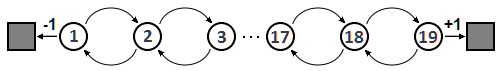
\includegraphics[keepaspectratio=true, width=0.9\textwidth]{\main/img/19_state_rw}
    \caption[19-State Random Walk] {
    The 19-state random walk environment. 
    Reaching the leftmost state results in a reward of $-1$, whereas the rightmost state results in a reward of $+1$.
    Reaching either of these two states terminates the episode.
    }
    \label{fig:19staterw}
\end{figure}

We will approach this task as an on-policy prediction problem.
At every time step, the agent follows and estimates the action-values corresponding to a fixed policy that with equal probability chooses between the left or right actions.
The benefit of using this type of environment is that it is possible to compute analytically the exact action-value function for each state.
We can then use this information to assess the accuracy of the action-value functions computed by the $n$-step $Q(\sigma)$ algorithm at different times during training.
The performance measure that we used for this experiment is the root-mean-squared (RMS) error between the true and the estimated action-value function.

We implemented $Q(\sigma)$ agents for each values of $\sigma$ from $0$ to $1$ at increments of $0.25$.
% in $\{0, 0.25, 0.5, 0.75, 1\}$.
For each of these algorithms, we optimized over the learning rate $\alpha$ and the backup length $n$ for the best performance in terms of the RMS error over 50 episodes of training. 
For all the algorithms, the best parameter combination was $n = 3$ and $\alpha = 0.4$.

$Q(1)$ (Sarsa) performed the best among all the other algorithms early during training, whereas $Q(0)$ (tree backup) performed the best at the end of training.
As the value of $\sigma$ decreased from $1$ to $0$, the corresponding algorithms performed worse during early training and better during late training.

These results support our initial hypothesis and the intuition developed in chapter \ref{ch4:convergence}.
It seems that using a value of $\sigma$ close to $1$ reduces the bias during early training, whereas a value of $\sigma$ close to $0$ reduces the bias during late training.

Given these conclusions, it seemed possible to device an algorithm that benefits from the initial performance induced by a value of $\sigma$ close to $1$ and the final performance induced by a value of $\sigma$ close to $0$.
We decided to test this idea by extending the experiment to include another $n$-step $Q(\sigma)$ algorithm.
For this instance of the $n$-step $Q(\sigma)$ algorithm, the parameter $\sigma$ is initialized at a value of $1$ and slowly decays to $0$ by a factor $\beta \in [0,1)$ at the end of each episode.
Specifically, we let $\sigma_{k+1} = \beta \cdot \sigma_k$ for $k \geq 1$ and $\sigma_1 = 1$.
We originally called this algorithm \textit{Dynamic} $\sigma$; however, I will use the name \textit{Decaying} $\sigma$ since it is more faithful to the true nature of the algorithm.
We hypothesized that using this simple heuristic, the algorithm would be able to perform the best during early and late training.

We implemented a decaying $\sigma$ algorithm with decay rate $\beta$ of $0.95$ and optimized over the parameters $n$ and $\alpha$.
The best parameter combination for decaying $\sigma$ was the same as for the other algorithms, $n = 3$ and $\alpha = 0.4$.

Compared to the algorithms from the first part of this experiment, decaying $\sigma$ performed the best at every stage of learning.
Figure \ref{fig:19staterw_plot} shows the RMS error computed at the end of each episode for each algorithm. 
The results are averaged over 100 runs.
All the standard errors are less than 0.006, which is narrower than the line width.

\begin{figure}[t]
    \centering
    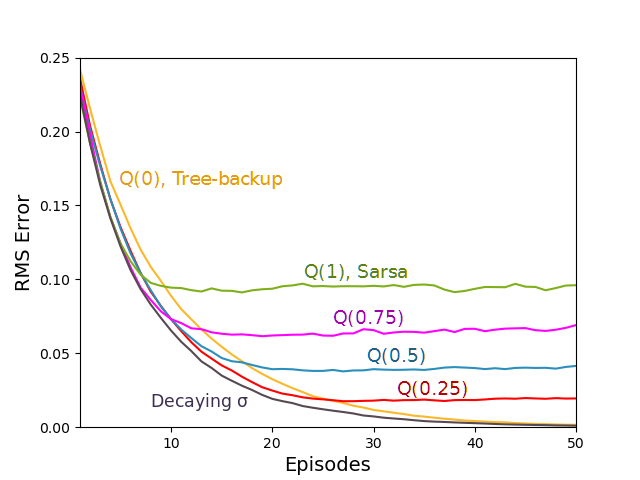
\includegraphics[keepaspectratio=true, width=0.9\textwidth]{\main/img/19_state_rw_plot}
    \caption[Results of the 19-State Random Walk Experiment] {
    Results of the 19-state random walk experiment. 
    Small values of $\sigma$ resulted in better initial performance in terms of root-mean-squared (RMS) error.
    Larger values of $\sigma$ resulted in better final performance.
    Decaying $\sigma$ with decay rate of 0.95 outperformed all the other variants of $Q(\sigma)$ with fixed value of $\sigma$.
    }
    \label{fig:19staterw_plot}
\end{figure}

% The results of this experiment show that, for this domain, the initial performance of the $n$-step $Q(\sigma)$ algorithm improved as the value of $\sigma$ increases from zero to one.
% On the other hand, the final performance decreased as $\sigma$ increased.
% The Decaying $\sigma$ algorithm seemed to be able to take advantage of these two effects by starting with a high $\sigma$ early during training and decaying over time towards a small $\sigma$.

It seems that, for this particular domain, the decaying $\sigma$ algorithm is taking advantage of the initial performance induced by high values of $\sigma$ and the final performance corresponding to small values of $\sigma$.
This supports our hypothesis about the decaying $\sigma$ algorithm and further supports the intuition developed in the previous chapter.
A value of $\sigma$ close to one makes the estimate of the return less bias early during training.
As training progresses and the estimates of the action-value function become more accurate, a small value of $\sigma$  results in less bias.
We encounter evidence of this effect several times during this chapter.

%%%%%%%%%%%%%%%%%%%%%%%%%%%%%%%%%%%%%%
%%%%% Stochastic Windy Gridworld %%%%%
%%%%%%%%%%%%%%%%%%%%%%%%%%%%%%%%%%%%%%
\section{$n$-Step Q($\sigma$) for On-Policy Control}

\begin{figure}[t]
    \centering
    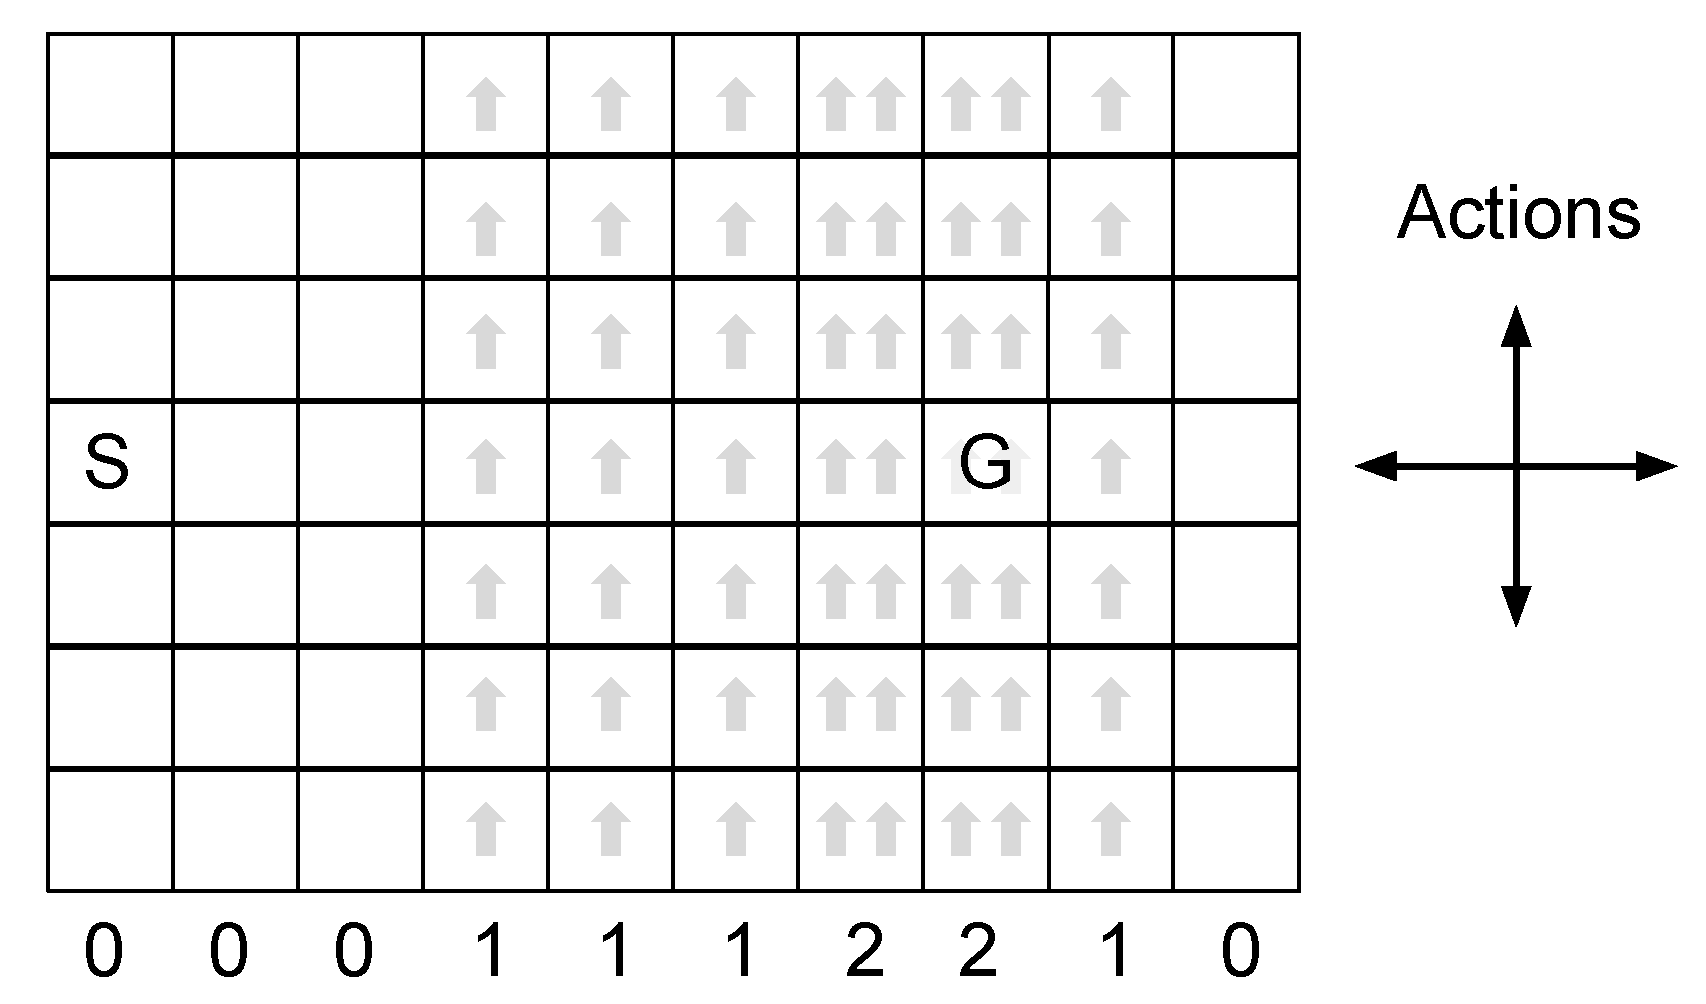
\includegraphics[keepaspectratio=true, width=0.9\textwidth]{\main/img/windy_gridworld}
    \caption[The Windy Gridworld Environment] {
    The windy gridworld environment.
    The agent starts at state S and its goal is to reach the terminal state G.
    The actions available are moving north, east, south, and west.
    At every column in the grid there is an upward wind that pushes the agent north $k$ number of squares as indicated at the bottom of each column.
    The reward is -1 at every transition until the agent reaches state G.
    }
    \label{fig:windy_gridworld}
\end{figure}

In this experiment, we will increase the complexity of the learning task and study how the parameters $\sigma$, $n$, and $\alpha$ interact with each other and influence the performance of $n$-step $Q(\sigma)$.
Based on the results of the previous experiment, We hypothesized that the decaying $\sigma$ algorithm would perform the best over a wide variety of settings of the parameters $n$ and $\alpha$.
To test this hypothesis, we set up the learning problem as an on-policy control task in a variant of the windy gridworld environment \parencite{harm-hado-expected-sarsa, Sutton:1998:IRL:551283}.

In the windy gridworld environment (figrue \ref{fig:windy_gridworld}), states are represented as discrete $(x,y)$ coordinates indicating the position of the agent in a grid enclosed within $4$ walls.
The actions available to the agent are moving north, east, south, or west.
At every column in the grid there is an upward wind that pushes the agent north $k$ number of squares after an action has been selected and executed.
After every action, the agent receives a reward of $-1$.
When an agent tries to move against a wall it stays in the same location, but executing the action still results in a reward of $-1$.
The agent starts at an initial state S and an episode terminates only when the agent moves into a goal state G.
Consequently, in order to maximize reward, the agent has to learn how to navigate the gridworld while accounting for the effects of the wind.

For this experiment, We used a variant of the windy gridworld environment called stochastic windy gridworld.
In this variant, all the details of the environment are the same except for the way that actions are executed.
In the stochastic windy gridworld, the agent moves to the desired direction only with a probability of $0.9$.
Otherwise, the agent is moved into one of the eight adjacent squares chosen uniformly at random.
The effect of the wind occurs after the action has been selected and executed just as in the original environment.

In order to study the effects of the parameters $\sigma$, $n$, and $\alpha$, we implemented eighty different $Q(\sigma)$ agents.
For each value of $n$ in $\{1 , 3\}$, we implemented four $Q(\sigma)$ agents, one for each value of $\sigma$ in $\{0, 0.5, 1\}$ and a decaying $\sigma$ agent with decay rate of $0.95$.
For each of these settings, we trained an agent for each value of $\alpha$ from $0.1$ to $1$ at increments of $0.1$. 
All the agents used an $\epsilon$-greedy policy with $\epsilon = 0.1$.
The measure of performance we used was the average return per episode over 100 episodes.

\begin{figure}[t]
    \centering
    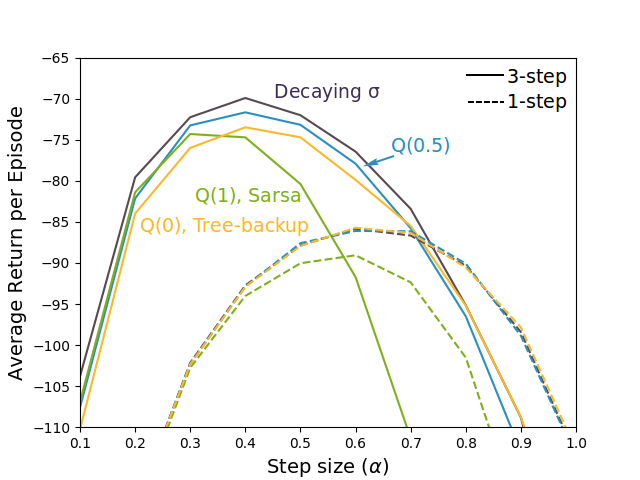
\includegraphics[keepaspectratio=true, width=0.9\textwidth]{\main/img/stochastic_windy_gridworld_results}
    \caption[Results of the Experiment on the Stochastic Windy Gridworld] {
    Results of the Experiment on the Stochastic Windy Gridworld.
    The results are averaged over 1000 runs of 100 episodes each.
    The standard error is narrower than the line width.
    The best performance for all the algorithms was achieved for a backup length, $n$, with value of three.
    For this backup length, Decaying $\sigma$ and $Q(0.5)$ have a better performance than Sarsa and Tree backup over a wide range of values of $\alpha$.
    }
    \label{fig:stochastic_wind_gridworld_results}
\end{figure}

For a back up length of $1$, $Q(0.5)$, $Q(0)$ and decaying $\sigma$ performed the same across all values of $\alpha$, while $Q(1)$'s performance was lower at most values of $\alpha$.
For a backup length of $3$, for most of the values of $\alpha$ the resulting performance was higher than for a backup length of $1$ across all the settings for $\sigma$.
In this latter case, $n = 3$, decaying $\sigma$ performed better than the algorithms with fixed $\sigma$ for most of the values of $\alpha$.
The parameter combination that resulted in the best performance was $n = 3$ and $\alpha = 0.4$ for decaying $\sigma$, $Q(0.5)$, and $Q(0)$; and $n = 3$ and $\alpha = 0.3$ for $Q(1)$.
Comparing only the best parameter combination of each algorithm we observed that decaying $\sigma$ performed the best with $Q(0.5)$ as a close second.

Figure \ref{fig:stochastic_wind_gridworld_results} shows the average return per episode over 100 episodes.
The results are averaged over $1,000$ independent runs of $100$ episodes each.
The error bars corresponding to the standard error are narrower than the line width.

The results of the experiment partially support the initial hypothesis.
Decaying $\sigma$ performed better than the rest of the algorithms for a wide variety of values of $\alpha$ when the backup length was $3$.
However, this was not the case for a backup length of $1$, in which case decaying $\sigma$, $Q(0.5)$, and $Q(0)$ performed the same.
Lastly, for $n=3$, $Q(0.5)$  also managed to outperform $Q(0)$ and $Q(1)$ demonstrating that intermediate values of $\sigma$ can also perform better than either of the extremes.
We find similar effects in more complex environments when using function approximation in the next sections of this chapter.

%%%%%%%%%%%%%%%%%%%%%%%%%%%%%%%%%%%%%%
%%%%% Mountain Cliff Experiment  %%%%%
%%%%%%%%%%%%%%%%%%%%%%%%%%%%%%%%%%%%%%
\section{$n$-Step Q($\sigma$) with Linear Function Approximation}

We will continue increasing the complexity of the learning task to study how robust are the results from the previous two experiments.
In this case, we study the performance of $n$-step $Q(\sigma)$ in a continuous task with linear function approximation.
Our goal in this experiment was to investigate if the effects found in the tabular case carry over to the linear function approximation case.
We hypothesized that there would be similar effects as in the tabular case: (1) decaying $\sigma$ would perform the best, and (2) higher values of the parameter $\sigma$ would perform better during early training, whereas lower values would perform better during late training.
We studied these hypotheses in an on-policy control task in a variant of the mountain car environment that we named \textit{mountain cliff} \parencite{Sutton:1998:IRL:551283}.

\begin{figure}[t]
    \centering
    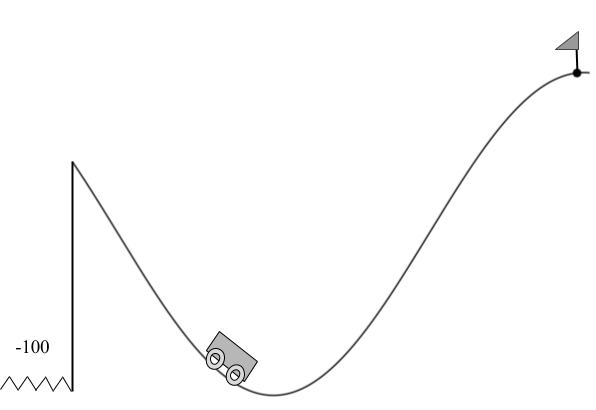
\includegraphics[keepaspectratio=true, width=0.8\textwidth]{\main/img/mountain_cliff}
    \caption[The Mountain Cliff Environment] {
    The mountain cliff environment. 
    The agent controls a car that is located between two hills.
    The goal is to reach the top of the right hill.
    The state is represented as a tuple containing the current position and velocity of the car.
    The actions are accelerating forward, backwards, or coasting.
    The agent receives a reward of -1 on every transition and a reward of -100 when it falls off the cliff at the top of the left hill.
    In the latter case, the agent is returned to a random location in the valley between the two hills with a velocity of zero.
    }
    \label{fig:mountain_cliff}
\end{figure}

In the mountain cliff environment (figure \ref{fig:mountain_cliff}) states are represented by a tuple of two continuous numbers that represent the position and the velocity of a car that is located in the valley between two hills.
The actions available to the agent are: accelerate forward $(+1)$, accelerate backwards $(-1)$, or coast.
Every action results in a reward of $-1$ and changes the position $x_t$ and the velocity $y_t$ of the car according to the simplified physics model:
%% Mountain Cliff Physics
\begin{align}
\label{eq:mountain_cliff_phys}
    y_{t+1} & \overset{.}{=} \textit{bound}\big[ y_t  + 0.001 A_t - 0.0025 \cos{3 x_t}  \big],
    \nonumber \\
    x_{t+1} & \overset{.}{=} \textit{bound}\big[ x_t + y_{t+1} \big],
\end{align}
%
where the \textit{bound} operation enforces $x_{t} \in [-1.2, 0.5]$ and $y_t \in [-0.07, 0.07]$.
The initial state of every episode is initialized to a random position in the interval $[-0.6, -0.4)$ and with zero velocity.
If an agent ever moves beyond the top of the left hill (position $-1.2$), it falls off a cliff, receives a reward of $-100$, and is sent to a random state chosen in the same way as the initial state.
On the other hand, once the agent's reaches the top of the right hill (position $0.5$) the episode terminates.
Consequently, maximizing reward implies reaching the top of the right hill as fast as possible.
However, the engine of the car is not strong enough to overcome the force of gravity.
Hence, the agent has to build momentum by moving back and forth in order to reach the top of the right hill without falling off the cliff at the end of the left hill.

The only difference between the mountain car and mountain cliff environments is the cliff at the end of the left hill.
In mountain car moving beyond the top of the left hill stops the movement of the agent and resets its velocity back to zero.
In comparison, the outcome in this same situation in the mountain cliff environment is a lot more punishing to the agent. 
Hence, the agent has to be more precise when moving onto the left hill.
The consequence of this environment design choice is that the difference in performance between different algorithms is accentuated, which facilitates their comparison.
All the agents were trained for $500$ episodes in this environment.

In order to study the effects of the parameter $\sigma$ on the performance of the $n$-step $Q(\sigma)$ algorithm we implemented six different agents: one for each value of $\sigma$ in $\{ 0, 0.25, 0.5, 0.75, 1\}$ and a decaying $\sigma$ agent with decay rate of $0.95$.
All the agents, were trained on-policy using an $\epsilon$-greed policy with $\epsilon = 0.1$.
The action-value was approximated using linear function approximation with tile coded features.
The tile coder was made up of 32 tilings with asymmetric offset and with each tiling covering $1/8$-th of the bounded distance in each dimension.
Using this configuration, the total number of parameters used by the function approximator was $6,144$.

The performance measure that we used in this task was the average return per episode.
To study the initial performance we used the first 50 episodes to compute the average return per episode, whereas for the final performance we used the last 50 episodes of training.
To study the overall performance of the algorithm we looked at the average return per episode over 500 episodes.
We optimized for the overall performance over the parameters $n$ and $\alpha$ in order to find the best parameter combination for each algorithm.
Decaying $\sigma$, $Q(0)$, $Q(0.25)$, and $Q(0.5)$ performed the best with $n = 4$ and $\alpha = 1/3$; $Q(0.75)$ performed the best with $n = 3$ and $\alpha = 1/3$; and $Q(1)$ performed the best with $n = 3$ and $\alpha = 1/4$. 
These values of $\alpha$ correspond to the values before dividing by the number of tilings used in the tile coder.

In terms of initial performance, the decaying $\sigma$ algorithm performed the best followed by $Q(0.5)$.
The initial performance decreased as the value of $\sigma$ moved away from $0.5$.
In terms of final performance, decaying $\sigma$ and $Q(0)$ performed the best followed closely by $Q(0.25)$.
As the value of $\sigma$ increased from $0$ to $1$, the final performance of the corresponding algorithms decreased with $Q(1)$ having the worst final performance.
Table \ref{tbl:mountain_cliff_results} shows the summary of the initial and final performance for all the algorithms.

\begin{table}[t] 
\caption[Experiment Results in the Mountain Cliff Environment in Terms of Initial and Final Performance]{
Summaries of the average return over the first and last 50 episodes for each algorithm.
The standard error, and lower (LB) and upper (UB) 95\% confidence interval bounds are provided to validate the results.
Decaying $\sigma$ had the best initial.
Decaying $\sigma$ and Tree Backup tied for the best final performance.
}
\label{tbl:mountain_cliff_results}
\begin{center}
\begin{tabular}{lcccc}
\toprule
& \multicolumn{4}{c}{Average Return of First 50 Episodes} \\
\cmidrule{2-5}
Algorithm & Mean & Standard Error & LB & UB \\
\midrule
$Q(1)$, Sarsa 		& -402.25           & 0.52  & -401.23           & -403.26   \\
$Q(0.75)$  			& -366.63           & 0.49  & -365.66           & -367.59   \\
$Q(0.5)$  			& -352.88           & 0.56  & -351.79           & -353.98   \\
$Q(0.25)$  			& -355.44           & 0.54  & -354.38           & -356.5    \\
$Q(0)$, Tree-backup & -362.48           & 0.54  & -361.43           & -363.54   \\
Decaying $\sigma$ 	& \textbf{-346.44}  & 0.60  & \textbf{-345.26}  & \textbf{-347.63}   \\
\bottomrule
&&&& \\
\toprule
& \multicolumn{4}{c}{Average Return of Last 50 Episodes} \\
\cmidrule{2-5}
Algorithm & Mean & Standard Error & LB & UB \\
\midrule
$Q(1)$, Sarsa 		& -134.41           & 0.20  & -134.02	        & -134.8    \\
$Q(0.75)$  			& -132.33           & 0.18  & -131.99	        & -132.68   \\
$Q(0.5)$  			& -131.44           & 0.26  & -130.94	        & -131.95   \\
$Q(0.25)$  			& -127.5            & 0.16  & -127.18	        & -127.82   \\
$Q(0)$, Tree Backup & \textbf{-126.7}   & 0.15  & \textbf{-126.41}	& \textbf{-126.99} \\
Decaying $\sigma$ 	& \textbf{-126.96}  & 0.15  & \textbf{-126.66}  & \textbf{-127.26}  \\
\bottomrule
\end{tabular}
\end{center}
\end{table}

In terms of overall performance, decaying $\sigma$ performed the best among all the algorithms closely followed by $Q(0.25)$.
$Q(0)$ (tree backup) performed the third best among all the algorithms, while $Q(1)$ (Sarsa) performed the worst.
The summary of the overall performance for all the algorithms can be seen in table \ref{tbl:mountain_cliff_total_results}.

\begin{table}[t] 
\caption[Experiment Results in the Mountain Cliff Environment in Terms of Average Return After 500 Episodes]{Summaries of the performance of each algorithm in terms of average return per episode over 500 episodes. 
The standard error, and lower (LB) and upper (UB) 95\% confidence interval bounds are provided to validate the results.
Under this measure of performance, Decaying $\sigma$ achieved the best performance followed closely by $Q(0.25)$.
}
\label{tbl:mountain_cliff_total_results}
\begin{center}
\begin{tabular}{lcccc}
\toprule
& \multicolumn{4}{c}{Average Return Over 500 Episodes} \\
\cmidrule{2-5}
Algorithm & Mean & Standard Error & LB & UB \\
\midrule
$Q(1)$, Sarsa 		& -164.34	        & 0.06	& -164.46	        & -164.22   \\           
$Q(0.75)$  			& -158.87	        & 0.06	& -158.98	        & -158.76   \\
$Q(0.5)$  			& -155.7	        & 0.07	& -155.84	        & -155.57   \\
$Q(0.25)$  			& -153.74	        & 0.06	& -153.85	        & -153.63   \\
$Q(0)$, Tree Backup & -154.11	        & 0.06	& -154.23	        & -153.99   \\
Decaying $\sigma$ 	& \textbf{-152.56}	& 0.06	& \textbf{-152.68}	& \textbf{-152.43}   \\
\bottomrule
\end{tabular}
\end{center}
\end{table}

Figure \ref{fig:mountain_cliff_results} shows the performance of all the algorithms at intervals of $50$ episodes.
The results are the average over $1,500$ independent runs and the error bars correspond to a $95\%$ confidence interval computed using a t-distribution.

\begin{figure}[t]
    \setlength{\abovecaptionskip}{0pt plus 0pt minus 0pt}
    \centering
    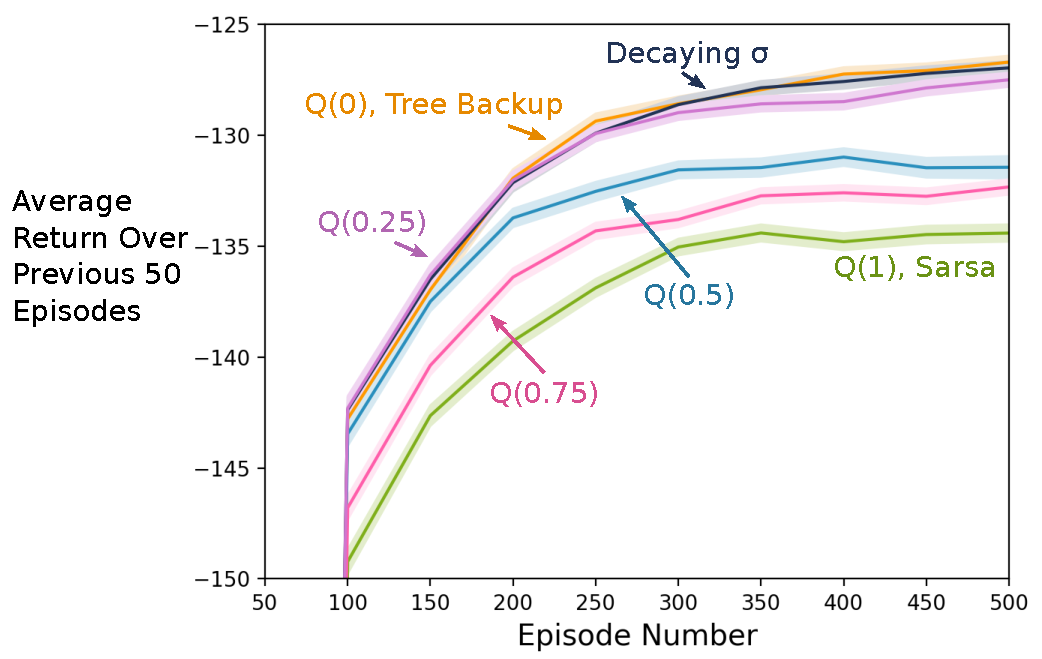
\includegraphics[keepaspectratio=true, width=1\textwidth]{\main/img/mountain_cliff_results}
    \caption[The Results of the Mountain Cliff Experiment] {
    The Results of the Mountain Cliff Experiment. 
    The plot shows the average return over the preceding 50 episodes.
    The shaded area corresponds to a 95\% confidence interval.
    These results correspond to the average over 1,500 independent runs.
    Decaying $\sigma$ and Tree Back up had very similar performance under this performance measure.
    As $\sigma$ increases, the final performance of the algorithm decreased, which is reminiscent to the 19-step random walk results.
    }
    \label{fig:mountain_cliff_results}
\end{figure}

The results support our first hypothesis since decaying $\sigma$ performed the best in terms of overall performance.
This further supports the idea that decaying $\sigma$ benefits from the initial performance induced by high values of $\sigma$ and from the final performance induced by small values of $\sigma$.
Moreover, once again we found an intermediate value of $\sigma$ that outperformed either of the extremes --- $Q(0.25)$.

On the other hand, these results partially support our second hypothesis.
It seems that in this more complex environment the effect of $\sigma$ on the initial performance is not linear.
Otherwise, we would observe that the initial performance increases steadily as $\sigma$ is increased from $0$ to $1$.
Nevertheless, it seems that it is possible to tune the parameter $\sigma$ in order to improve the initial performance of an algorithm.
In terms of final performance, we observed a similar pattern as in the 19-step random walk experiment: as $\sigma$ decreases the final performance improves.
However, it seems that the effect on the final performance is less pronounced as $\sigma$ gets closer to $0$.
We find evidence that supports the first hypothesis and that partially supports the second hypothesis when using non-linear function approximation.

%%%%%%%%%%%%%%%%%%%%%%%%%%%%%%%%%%%%%%
%%%%% Mountain Car Experiment  %%%%%
%%%%%%%%%%%%%%%%%%%%%%%%%%%%%%%%%%%%%%
\section{$n$-step $Q(\sigma)$ with Non-Linear Function Approximation: The Deep Q($\sigma$) Network}
\label{sec:dqsigman}

We continue increasing the complexity of the learning task by studying the performance of the $n$-step $Q(\sigma)$ algorithm when combined with the DQN architecture --- an architecture that we have named the deep $Q(\sigma)$ network.
Our goal is to investigate whether we can find evidence of the effects observed in the previous experiments when using non-linear function approximation.
We formulated two hypotheses based on the previous results: (1) the decaying $\sigma$ algorithm would perform better than algorithms with fixed $\sigma$, and (2) large values of $\sigma$ would result in better initial performance whereas small values would result in better final performance.

Before studying the two main hypotheses of this section we studied the effects that certain algorithmic details of the DQN architecture have on the performance of the deep $Q(\sigma)$ ,network.
We divide this study into two main sets of experiments: (1) experiments studying the effects of the DQN architecture on the performance of the deep $Q(\sigma)$ network, and (2) experiments studying the effects of the parameters $\sigma$ and $n$.
Then, we go back to study the main hypotheses of this section.

To run all this experiments we set up the learning problem as an control task in the mountain car environment.
The mountain car environment is set up as described in the previous section.
We decided against using the mountain cliff environment because it added extra noise to the results and took longer to learn.
Moreover, the DQN architecture clips the rewards so that their values are between $-1$ and $1$; hence, implementing this algorithmic detail in the mountain cliff environment would eliminate the punishing effect of the cliff.
We also imposed a timeout of $5,000$ steps in order to prevent episodes from running forever and overpopulating the experience replay buffer with observations that are too similar to each other.
It is important to note that timing out is not treated the same way as termination.
In the case of termination, all the subsequent rewards and action-value functions after the terminating state are considered zero.
In the case of a timeout, the return is computed by bootstrapping off of the last available action-value functions, effectively making the $n$-step estimate of the return shorter.
All the agents were trained for $500$ episodes in this environment.

\begin{table}[t]
    \centering
    \begin{tabular}{l|c|l}
        %%% Header %%%
         Hyperparameter                 & Value     & Description  \\ \bottomrule
         %% line 1: stepsize
         Step-size ($\alpha$)           & 0.00025   & Step-size used with RMSprop 
         \\ \hdashline[3pt/3pt]
         %% line 2: momentum
         Gradient momentum              & 0.95      & Gradient momentum used by RMSprop
         \\ \hdashline[3pt/3pt]
         %% line 3: squared gradient momentum
         Squared gradient               & 0.95      & Squared gradient (denominator)  \\
         momentum                       &           &  momentum used by the RMSprop  
         \\ \hdashline[3pt/3pt]
         %% line 4: min squared gradient
         Min squared                    & 0.01      & Connstant added to the denominator \\
         gradient                       &           & of the RMSprop update 
         \\ \hdashline[3pt/3pt]
         %% line 5: discount factor
         Discount factor ($\gamma$)     & 1.0       & Discount factor used in the $n$-step $Q(\sigma)$ \\
                                        &           & update
        \\ \hdashline[3pt/3pt]
        %% line 6: exploration rate
        Exploration rate ($\epsilon$)   & 0.1       & Probability that a random action will be \\
                                        &           & taken at each time step
        \\ \hdashline[3pt/3pt]
        %% line 7: minibatch size
        Minibatch size                  & 32        & Number of samples of the estimate of  \\
                                        &           & the return used to compute an update
        \\ \hdashline[3pt/3pt]
        %% line 8: replay memory
        Replay memory                   & 20,000    & Number of observations stored in the \\
                                        &           & experience replay buffer
        \\ \hdashline[3pt/3pt]
        %% line 9: replay start size
        Replay start size               & 1,000     & A random policy is ran for this many \\
                                        &           & time steps to populate the buffer 
        \\ \hdashline[3pt/3pt]
        %% line 10: update frequency
        Target network                  & 1,000     & Frequency --- measured in number of  \\
        update frequency*               &           & updates --- with which the target    \\
                                        &           & network is updated                    
        \\ \bottomrule
    \end{tabular}
    \caption[Hyperparameters for the Deep $Q(\sigma)$ Network Architecture]{The hyperparameters for the deep $Q(\sigma)$ network architecture.
    All the parameters remained fixed throughout this set of experiment except for the ones marked with an asterisk (*).
    }
    \label{tab:dqsigman_parameters}
\end{table}

We implemented the deep $Q(\sigma)$ network architecture as described in section (\ref{sec:dqsigman}).
All the agents in this set of experiments used the same network architecture consisting of an input layer, one hidden layer, and an output layer.
The input layer of the network consists of a state tuple containing the position and the velocity of the car at a given time step.
This input is passed to a fully-connected hidden layer that consists of 1000 rectified linear units.
The output of the hidden layer is fed into a fully connected linear layer that computes an estimate of the action-value function corresponding to each action.
The total number of parameters in the network is 6003.

The hyperparameters used by the deep $Q(\sigma)$ network are listed in table (\ref{tab:dqsigman_parameters}).
Most of the parameters for the deep $Q(\sigma)$ network architecture are the same as the ones used in the original DQN architecture.
We used the RMSprop optimizer to minimize the loss function as in the original DQN architecture \parencite{Tieleman2012, mnih2015humanlevel}.
The discount factor $\gamma$ was chosen to be one so that agents considered the full sequence of rewards in order to encourage them to find the terminal state before episodes timed out.
The replay memory size was selected by testing the performance of a DQN agent with a replay memory size of 100, 50, 20, and 5 thousand observations; it is important to emphasize that this was not an exhaustive search.
The target network update frequency and the replay start size were chosen to be 5\% of the size of the replay memory buffer.
All the hyper-parameters of the network remained fixed for all the experiments except for the target network update frequency.
We will make special emphasis when using a different value for the target network update frequency; otherwise, the reader should assume that the value of this hyperparameter is $1,000$.

The performance measure that we used in this task was the average return per episode.
We studied the initial performance by computing this measure over the first 50 episodes of training, whereas the final performance is computed in terms of the last 50 episodes of training.
The overall performance of the algorithm is computed using all the training episodes.

%%%%% Off-Policy vs On-Policy Sampling Experiment %%%%%
\subsection{Off-Policy vs On-Policy Sampling Experiment}

We start by studying the how sampling from the experience replay buffer affects the performance of the deep $Q(\sigma)$ network.
When sampling from the buffer one can correct for the difference between policy $\pi_k$, the policy used at the time a transition was stored in the buffer, and $\pi_t$, the policy used at the time a transition is sampled from the buffer.
This is equivalent to computing the importance sampling ratio $\frac{\pi_t(A_k|S_k)}{\pi_k(A_k|S_k)}$ in order to correct the sampling side of the $Q(\sigma)$ estimate of the return.
The expectation side of the estimate of the return does not have to be corrected since it already works off-policy.
Alternatively, one can choose to ignore this difference and hope that the bias of the return will not have a big effect on the performance of the algorithm.
We tested both solutions to the sampling problem.
Note that one solution corresponds to treating transitions as if they had been collected off-policy, while the second solution corresponds to considering transitions as if they were sampled on-policy.
Hence, we will refer to this sampling solutions as sampling off-policy vs on-policy.

The main goal of this experiment is to test if there is any difference in performance between these two sampling methods.
We hypothesized that sampling on-policy would perform better since the variance introduced by the importance sampling ratio would overcome the decrease in bias.

To test this hypothesis, we implemented an on-policy and an off-policy version of three different one-step $Q(\sigma)$ algorithms: $Q(1)$ (Sarsa), $Q(0.5)$, and a decaying $\sigma$ agent with decay rate of $0.95$.
We did not test $Q(0)$ (Expected Sarsa) since it works off-policy without using importance sampling.

$Q(1)$ and $Q(0.5)$ had better final and overall performance when sampling on-policy.
Across all the algorithms, sampling off-policy resulted in better initial performance.
The decaying $\sigma$ algorithm performed better when sampling off-policy in terms of initial, final, and overall performance.
The results of the experiment averaged over 100 independent runs with $95\%$ confidence intervals can be seen in figure (\ref{fig:off_policy_vs_on_policy_experiment}).

\begin{figure}[htp]
    \setlength{\abovecaptionskip}{5pt plus 0pt minus 0pt}
    \centering
    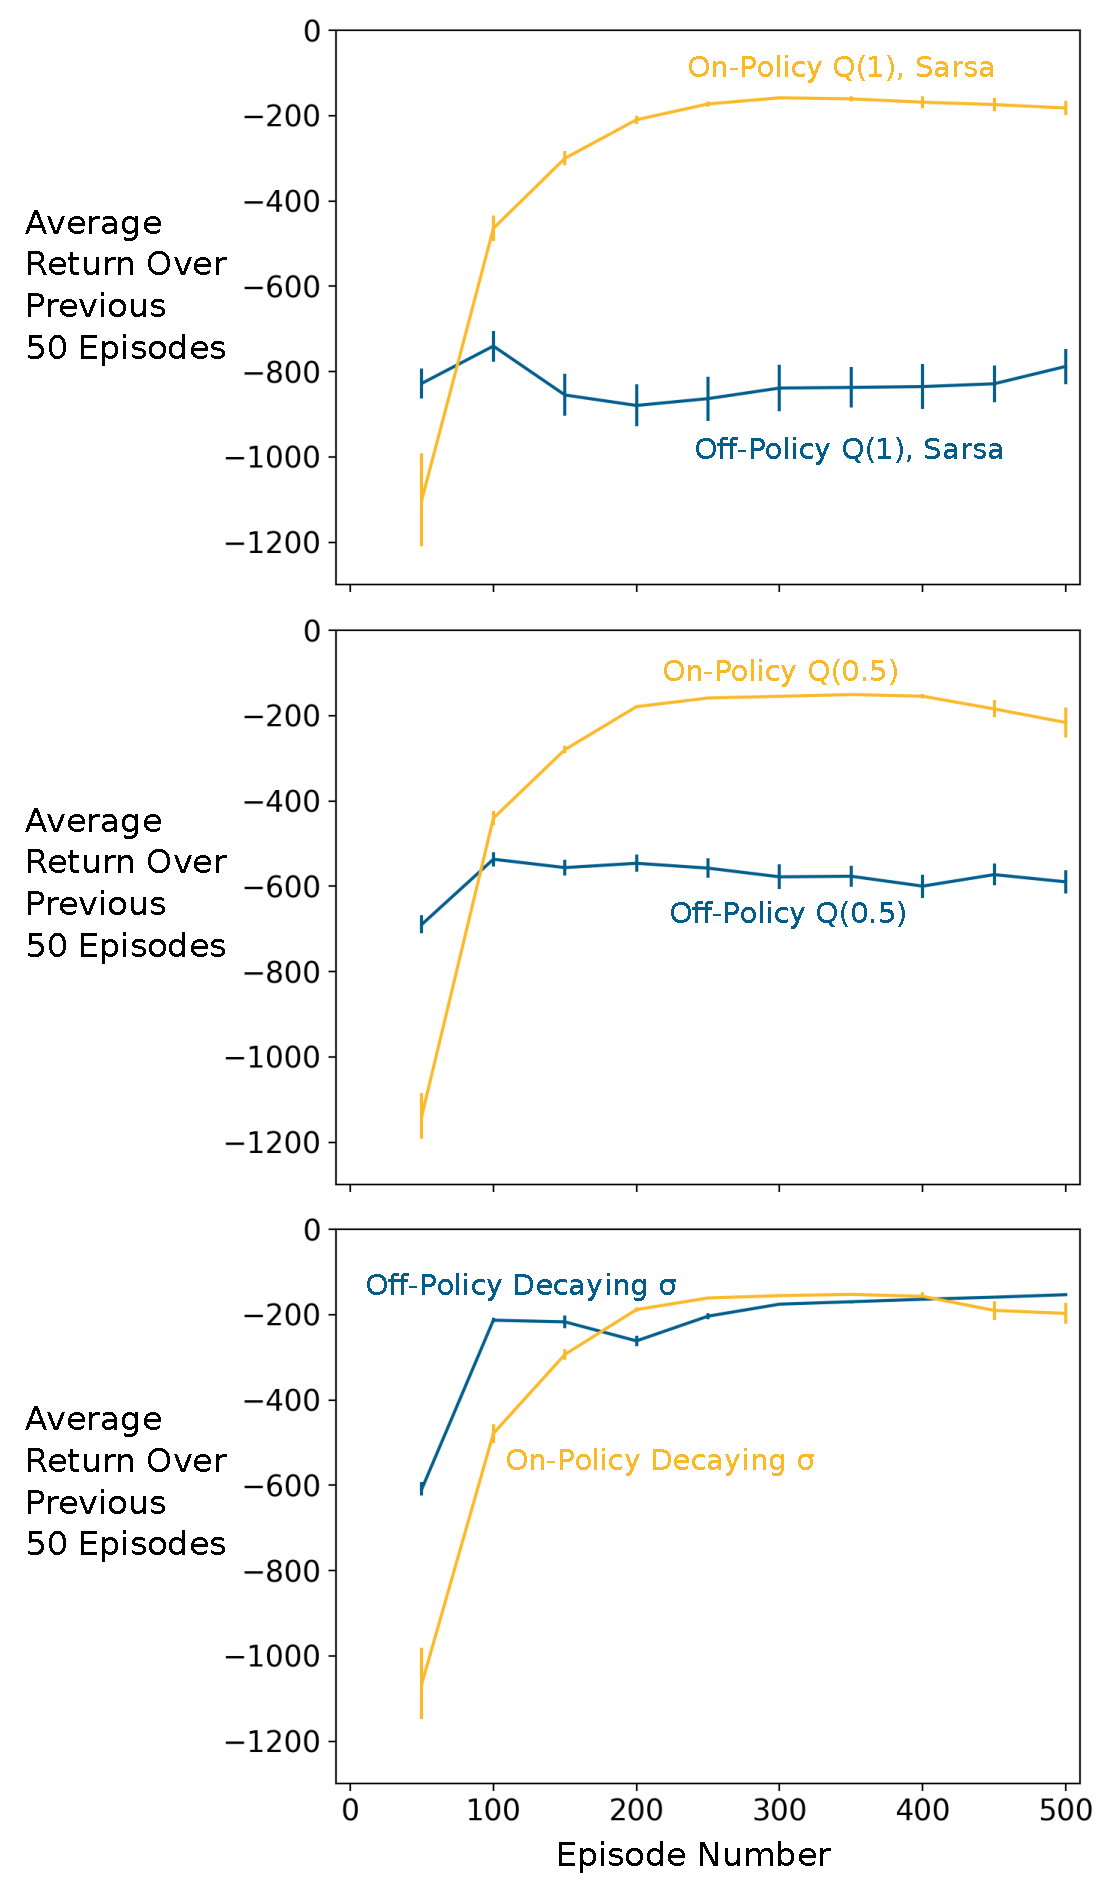
\includegraphics[keepaspectratio=true, width=0.8\textwidth]{\main/img/off_policy_vs_on_policy_results}
    \caption[Results of the Off-Policy vs On-Policy Experiment] {Results of the off-policy vs on-policy sampling experiment.
    The results are averaged over 100 independent runs.
    The error bars correspond to a 95\% confidence interval.
    Sarsa and $Q(0.5)$ (top and middle plots) have better performance when not using the importanc sampling ratio.
    On the other hand, dynamic $\sigma$ (bottom plot) benefited from using importance sampling ratio.
    }
    \label{fig:off_policy_vs_on_policy_experiment}
\end{figure}

The results of this experiment partially support our hypothesis.
For $Q(1)$ and $Q(0.5)$ sampling off-policy resulted in worse performance.
Additionally, the performance of these two algorithms consistently had higher variance --- as evidenced by the error bars of the plot.
This supports the claim that the importance sampling ratio added extra variance to the estimate of the return.

In the case of decaying $\sigma$ we observed the opposite effect: the off-policy algorithm performed considerably better.
This could be explained by the high decay rate of the algorithm.
Initially, the estimate of the return has inherently high variance; hence, adding more variance while reducing the bias of the estimate results in better performance.
However, by episode $51$, the value of $\sigma$ is approximately $0.08$ meaning that the sampling side of the return --- the one using importance sampling --- has a very small weight assigned to it.
Consequently, the performance of the decaying $\sigma$ algorithm is not affected by the increase in variance induced by the importance sampling ratio.

This second conclusion has an important implication that could be exploited when using $n$-step $Q(\sigma)$ in the off-policy setting.
Analogous to the parameter $\lambda$ in the ABQ$(\zeta)$ algorithm \parencite{rupam2017}, the parameter $\sigma$ could be used in order to counteract the increase in variance induced by the importance sampling ratio.

Henceforth, we use the on-policy sampling version of all the algorithms that we test since it results in better performance for most of them.

%%%%% Effect of the Parameters n and sigma on the Performance of DQ(sigma)N %%%%%
\subsection{Effect of the Parameter $n$ on the Performance of the Deep $Q(\sigma)$ Network}

We move on to study how the parameter $n$ affects the performance of the deep $Q(\sigma)$ network across several settings of the parameter $\sigma$
Given the previous results in the mountain cliff environment, we hypothesized that values of $n$ greater than $1$ would result in better performance, but using too high values of $n$ would have and adverse effect in performance.
In order to test this hypothesis, we implemented for each value of $n$ in $\{1,3,5,10,20\}$ four different $Q(\sigma)$ algorithms: $Q(1)$ (Sarsa), $Q(0.5)$, $Q(0)$ (Tree Backup), and decaying $\sigma$ with decay rate of $0.95$.

Across all the different $Q(\sigma)$ algorithms, increasing the value of the parameter $n$ consistently improved the initial performance of the corresponding algorithms.
For $Q(1)$, there was no statistical significance between final performance of the algorithm with $n = 3, 5, 10, 20$, and all of them performed better than when using $n = 1$. 
In terms of overall performance, $n = 20$ resulted in the best performance for $Q(1)$.
For $Q(0.5)$, there was no statistical significance between the final performance of the algorithm with $n = 10$ and $20$, and both of these settings outperformed $Q(0.5)$ with $n = 1, 3$ and $5$.
In terms of overall performance, $n = 20$ resulted in the best performance for $Q(0.5)$.
$Q(0)$ performed the best with $n = 20$ in terms of final and overall performance.
Lastly, decaying $\sigma$ performed the best with $n \geq 5$ in terms of final performance and with $n \geq 10$ in terms of overall performance. 
Figure \ref{fig:nstep_dqsigman_results} shows the results corresponding to the average over $100$ independent runs.
The error bars correspond to a $95\%$ confidence interval.

\begin{figure}[t]
    \setlength{\abovecaptionskip}{0pt plus 0pt minus 0pt}
    \centering
    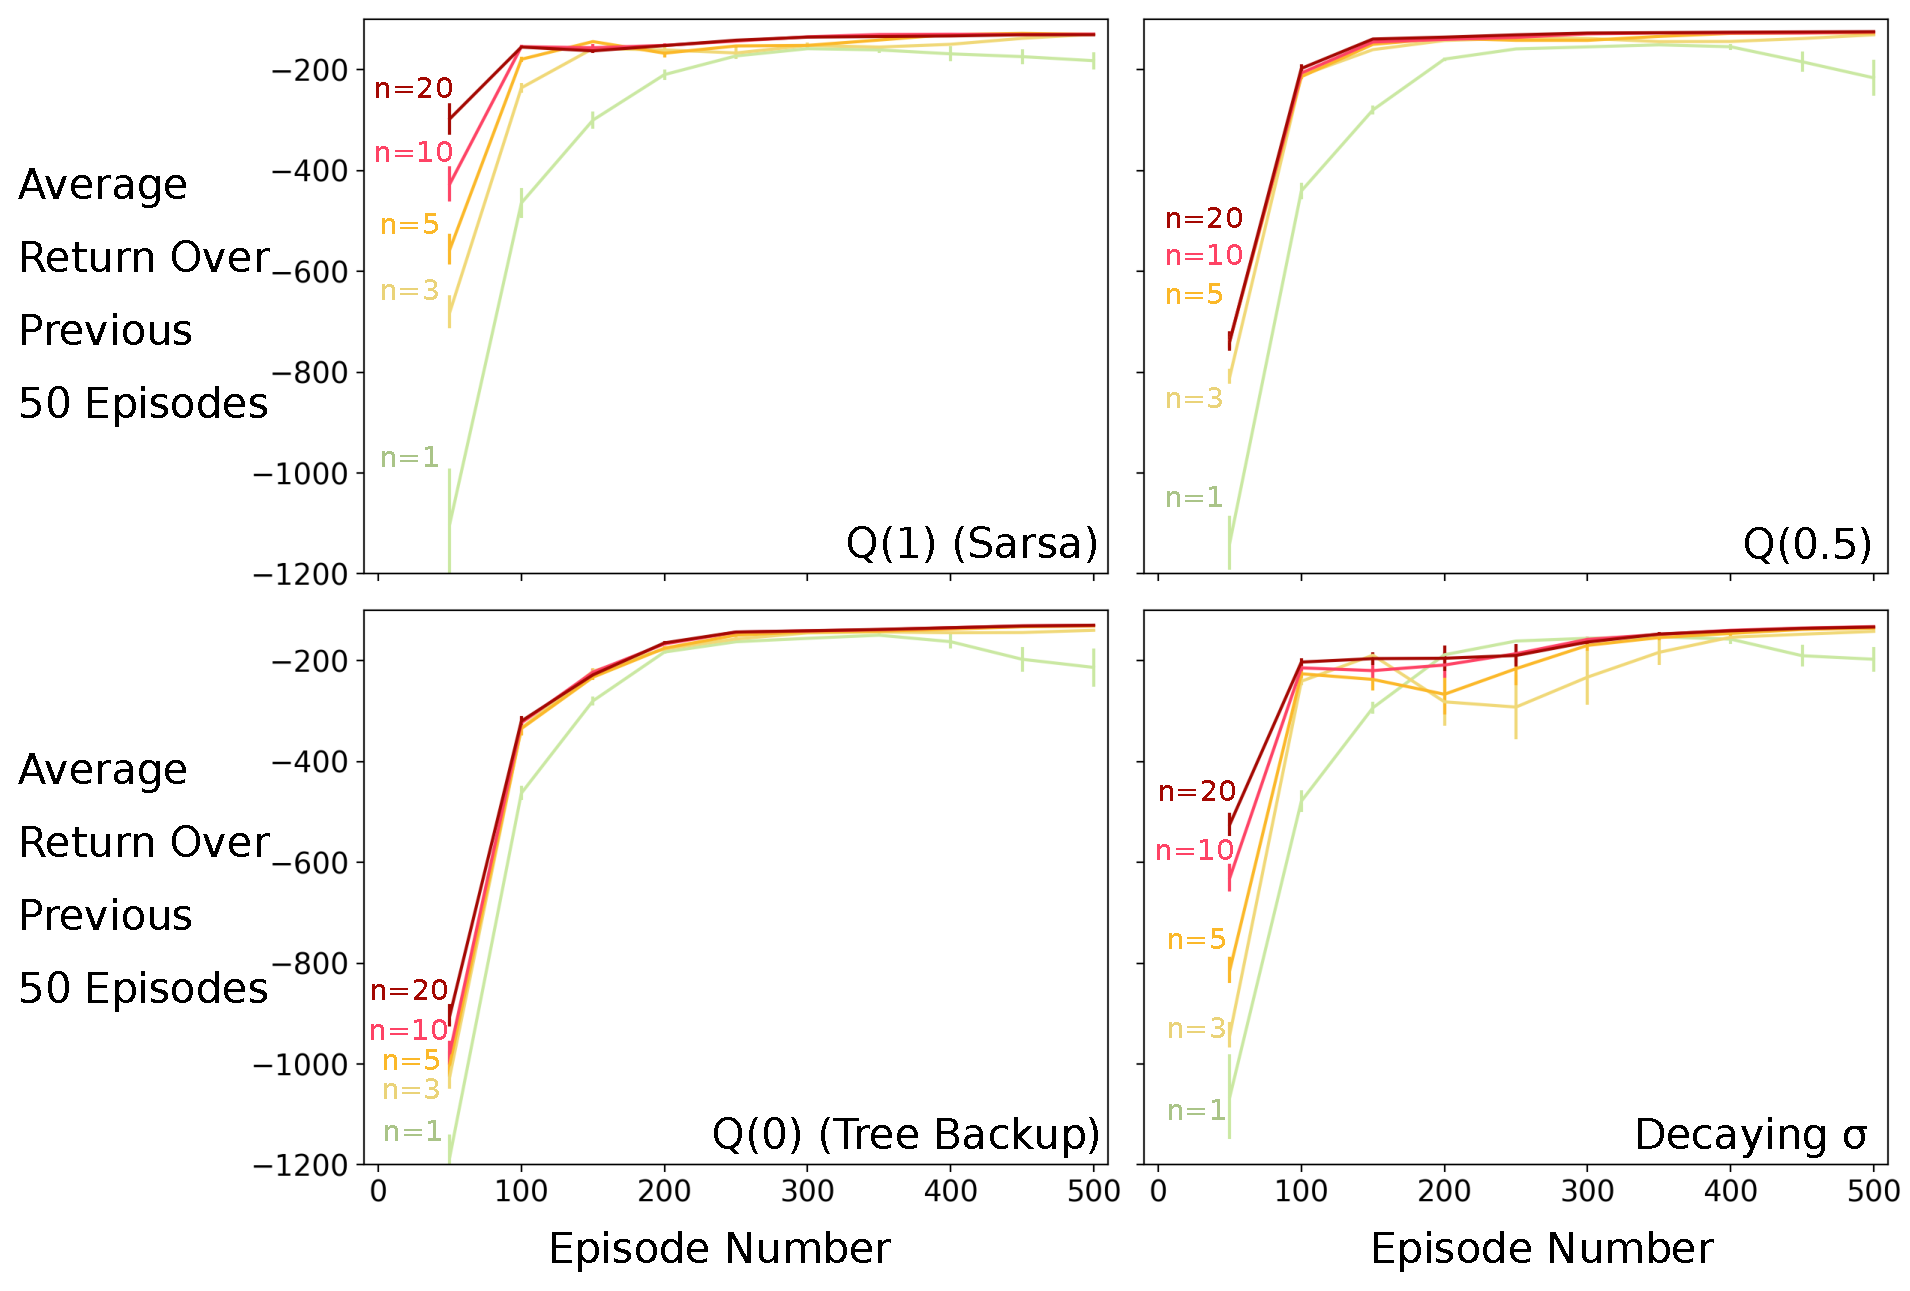
\includegraphics[keepaspectratio=true, width=1\textwidth]{\main/img/nstep_dqsigman_results}
    \caption[Performance of the Deep $Q(\sigma)$ Network for Different Values of $n$ and $\sigma$] {Performance of the deep $Q(\sigma)$ network for different values of $n$ and $\sigma$.
    The plots show the average over 100 independent runs with 95\% confidence intervals.
    All the algorithms benefit from having a larger back up length than one.
    The decaying $\sigma$ algorithm had less stable performance as evidenced by its high variance.
    }
    \label{fig:nstep_dqsigman_results}
\end{figure}

This results partially support our hypothesis: values of $n > 1$ performed better across all the algorithms, but we could not find a value of $n$ greater than $1$ that had an adverse effect on the performance of the algorithm.
Even though the initial performance for all the different $Q(\sigma)$ agents improved as $n$ increased, the magnitude of this effect was bigger the closer $\sigma$ was to $1$.
% For example, for $Q(1)$ the initial performance of the $1$-step algorithm was $-1,100.32 \pm 109.6$, whereas for the $20$-step version of $Q(1)$ it was $-297.2 \pm 31.32$.
% In contrast, for $Q(0)$ the initial performance of the $1$-step version was $-1183.69 \pm 43.08$, whereas the performance of the $20$-step version was $-903.61 \pm 22.17$.
% The parameter $n$ had a bigger effect in the initial performance of the algorithms with values of $\sigma$ closer to $1$.

% In terms of final performance, values of $n$ greater than $1$ resulted in different effects for different values of $\sigma$.
% For $Q(1)$, the $3$-step version had a final performance of $-129.47 \pm 1.91$, while the final performance of the $20$-step version was $-130.42 \pm 1.6$ --- the difference is not statistically significant.
% On the other hand, for $Q(0)$ the final performance of the $3$-step version was $-139.47 \pm 1.45$, whereas for the $20$-step version the final performance was $-129.47 \pm 0.83$.
% Decaying $\sigma$ and $Q(0.5)$ showed a similar pattern as $Q(0)$ with a smaller magnitude. 
% The parameter $n$ seemed to have a bigger effect in the final performance of the algorithms with values of $\sigma$ closer to $0$.

Most of the algorithms did not show a high variance or instability in their performance across different stages of training.
However, there were two special cases that stood out: one-step algorithms and decaying $\sigma$.
For all the one-step methods there was a dip in performance during the last one hundred episodes.
This did not happened for algorithms with $n$ greater than one.
However, it is not possible to determine from these results whether this dip in performance was completely avoided or whether it was just delayed to a time frame greater than the one we used.

In the case of decaying $\sigma$ the outstanding pattern is the drop in performance and increase in variance during the middle of training.
This happened with a bigger magnitude for smaller values of $n$ than higher values.
Moreover, this pattern happened across all values of $n$ except for $n=1$.
The pattern observed in the performance of the decaying $\sigma$ algorithm motivated the next two experiments.

%%%%% Effect of the decay rate on the performance of the deep $Q(\sigma)$ network %%%%%
\subsection{Effect of the Decay Rate on the Performance of the Deep $Q(\sigma)$ Network}

One possible explanation for the drop in performance experienced by the decaying $\sigma$ algorithm is that the loss function of the neural network is changing too fast making learning unstable.
This would also explain why at the end of training the performance stabilizes again.
Close to the end, the value of $\sigma$ is close to $0$ and the changes in the value of $\sigma$ are very small; consequently, the loss function barely changes episode by episode.
We hypothesized that if the decay rate was slower, then the drop in performance experienced by the decaying $\sigma$ algorithm would be smaller.

To test this hypothesis we implemented a second decaying $\sigma$ algorithm with a linear decay rate instead of an exponential decay rate for each value of $n$ in $\{3, 5, 10, 20\}$.
In this case, instead of multiplying $\sigma$ by a factor of $0.95$ at the end of each episode, we subtracted $0.002$ from the value of $\sigma$ after every episode.
We compared the performance of the linear and exponential decays and measured the severity of the drop in performance.

In order to gain a more detailed view of the performance of the algorithms in this experiment, we used a different time scale when plotting and analyzing the data.
We used the average return per episode as measure of performance; however, instead of looking at intervals of $50$ episodes, we decreased the size of the intervals to $10$ episodes.
In order to measure the severity of the drop in performance, we first looked at the $10$ episode interval before the start of the drop --- the start, and the $10$ episode interval with the lowest performance during the drop --- the lowest point.
Then, within each run, we computed the difference in performance between the start of the drop and the lowest point in the drop and computed the average difference along with a $95\%$ confidence interval using a t-distribution.
Statistical analysis on the average difference computed in this way is equivalent to a paired t-test where the variable under study is measured for each subject before and after certain treatment or event.
Because of the high variability of the estimates we had to increase the sample size from $100$ to $1,000$ in order to obtain significant results with $95\%$ confidence.

\begin{table}[t] 
\caption[Comparison of the Drop in Performance Experienced by the Decaying $\sigma$ Algorithm with Linear Decay vs Exponential Decay for $n = 3$ and $5$]{Comparison of the drop in performance experienced by the decaying $\sigma$ algorithm with linear decay vs exponential decay for $n = 3$ and $5$. 
The severity of the drop in performance is measured in terms of the average difference between the performance at the start and at the lowest point of the drop within each run.
Lower (LB) and upper (UB) 95\% confidence interval bounds are provided to validate the results.
Decaying $\sigma$ with linear decay had a less severe drop in performance than with exponential decay.
}
\label{tbl:exp_vs_lin_decay}
\begin{center}
\begin{tabular}{lcccc}
\toprule
& \multicolumn{4}{c}{Average Drop in Performance} \\
\cmidrule{2-5}
$n = 3$ & Mean & Standard Error & LB & UB \\
\midrule
Linear Decay 		& 62.49     & 8.45  & 45.9  & 79.07     \\
Exponential Decay   & 114.55    & 10.87 & 93.21 & 135.89    \\
&&&& \\
& \multicolumn{2}{c}{Start} & \multicolumn{2}{c}{Lowest Point}  \\
\cmidrule(l){2-3} \cmidrule(l){4-5}
Linear Decay        & \multicolumn{2}{c}{Episodes 151 - 160}   & \multicolumn{2}{c}{Episodes 221 - 230} \\
Exponential Decay   & \multicolumn{2}{c}{Episodes 111 - 120}   & \multicolumn{2}{c}{Episodes 181 - 190} \\
\bottomrule
&&&& \\
\toprule
& \multicolumn{4}{c}{Average Drop in Performance} \\
\cmidrule{2-5}
$n = 5$ & Mean & Standard Error & LB & UB \\
\midrule
Linear Decay 		& 38.37 & 5.47  & 27.63 & 49.12 \\
Exponential Decay   & 72.64 & 7.73  & 57.48 & 87.81 \\
&&&& \\
& \multicolumn{2}{c}{Start} & \multicolumn{2}{c}{Lowest Point}  \\
\cmidrule(l){2-3} \cmidrule(l){4-5}
Linear Decay        & \multicolumn{2}{c}{Episodes 121 - 130}   & \multicolumn{2}{c}{Episodes 181 - 190} \\
Exponential Decay   & \multicolumn{2}{c}{Episodes 109 - 110}   & \multicolumn{2}{c}{Episodes 161 - 170} \\
\bottomrule
\end{tabular}
\end{center}
\end{table}

For both decaying $\sigma$ algorithms with $n = 3, 5$ and $20$, using a linear decay resulted in a smaller drop in performance in terms of the difference between the performance at the start and at the lowest point of the drop.
For the decaying $\sigma$ algorithm with $n = 10$, using a linear decay resulted in a smaller drop, but the difference in the size of the drop was not significant at a $95\%$ confidence level.
It is likely that for $n = 10$ we can get similar results if we increase the sample size.
Additionally, decaying $\sigma$ with linear decay performed better than decaying $\sigma$ with exponential decay in terms of average return per episode over $500$ episodes.
The summary of these results averaged over $1,000$  independent runs and with corresponding $95\%$ confidence intervals can be seen in tables \ref{tbl:exp_vs_lin_decay} and \ref{tbl:exp_vs_lin_decay2}.
Figure \ref{fig:linear_vs_exponential} shows the training performance of the algorithms.


\begin{table}[t] 
\caption[Comparison of the Drop in Performance Experienced by the Decaying $\sigma$ Algorithm with Linear Decay vs Exponential Decay for $n = 10$ and $20$]{Comparison of the drop in performance experienced by the decaying $\sigma$ algorithm with linear decay vs exponential decay for $n = 10$ and $20$. 
The severity of the drop in performance is measured in terms of the average difference between the performance at the start and at the lowest point of the drop within each run.
Lower (LB) and upper (UB) 95\% confidence interval bounds are provided to validate the results.
Decaying $\sigma$ with linear decay had a less severe drop in performance than with exponential decay.
}
\label{tbl:exp_vs_lin_decay2}
\begin{center}
\begin{tabular}{lcccc}
\toprule
& \multicolumn{4}{c}{Average Drop in Performance} \\
\cmidrule{2-5}
$n = 10$ & Mean & Standard Error & LB & UB \\
\midrule
Linear Decay 		& 24.42 & 3.01  & 18.52 & 30.32 \\
Exponential Decay   & 43.46 & 5.32  & 33.01 & 53.9  \\
&&&& \\
& \multicolumn{2}{c}{Start} & \multicolumn{2}{c}{Lowest Point}  \\
\cmidrule(l){2-3} \cmidrule(l){4-5}
Linear Decay        & \multicolumn{2}{c}{Episodes 101 - 110}   & \multicolumn{2}{c}{Episodes 201 - 210} \\
Exponential Decay   & \multicolumn{2}{c}{Episodes  91 - 100}   & \multicolumn{2}{c}{Episodes 121 - 130} \\
\bottomrule
&&&& \\
\toprule
& \multicolumn{4}{c}{Average Drop in Performance} \\
\cmidrule{2-5}
$n = 20$ & Mean & Standard Error & LB & UB \\
\midrule
Linear Decay 		& 9.81  & 3.06  & 3.8   & 15.81 \\
Exponential Decay   & 46.65 & 4.83  & 37.19 & 56.12 \\
&&&& \\
& \multicolumn{2}{c}{Start} & \multicolumn{2}{c}{Lowest Point}  \\
\cmidrule(l){2-3} \cmidrule(l){4-5}
Linear Decay        & \multicolumn{2}{c}{Episodes  91 - 100}   & \multicolumn{2}{c}{Episodes 201 - 210} \\
Exponential Decay   & \multicolumn{2}{c}{Episodes 101 - 110}   & \multicolumn{2}{c}{Episodes 131 - 140} \\
\bottomrule
\end{tabular}
\end{center}
\end{table}

\begin{figure}[t]
    \setlength{\abovecaptionskip}{0pt plus 0pt minus 0pt}
    \centering
    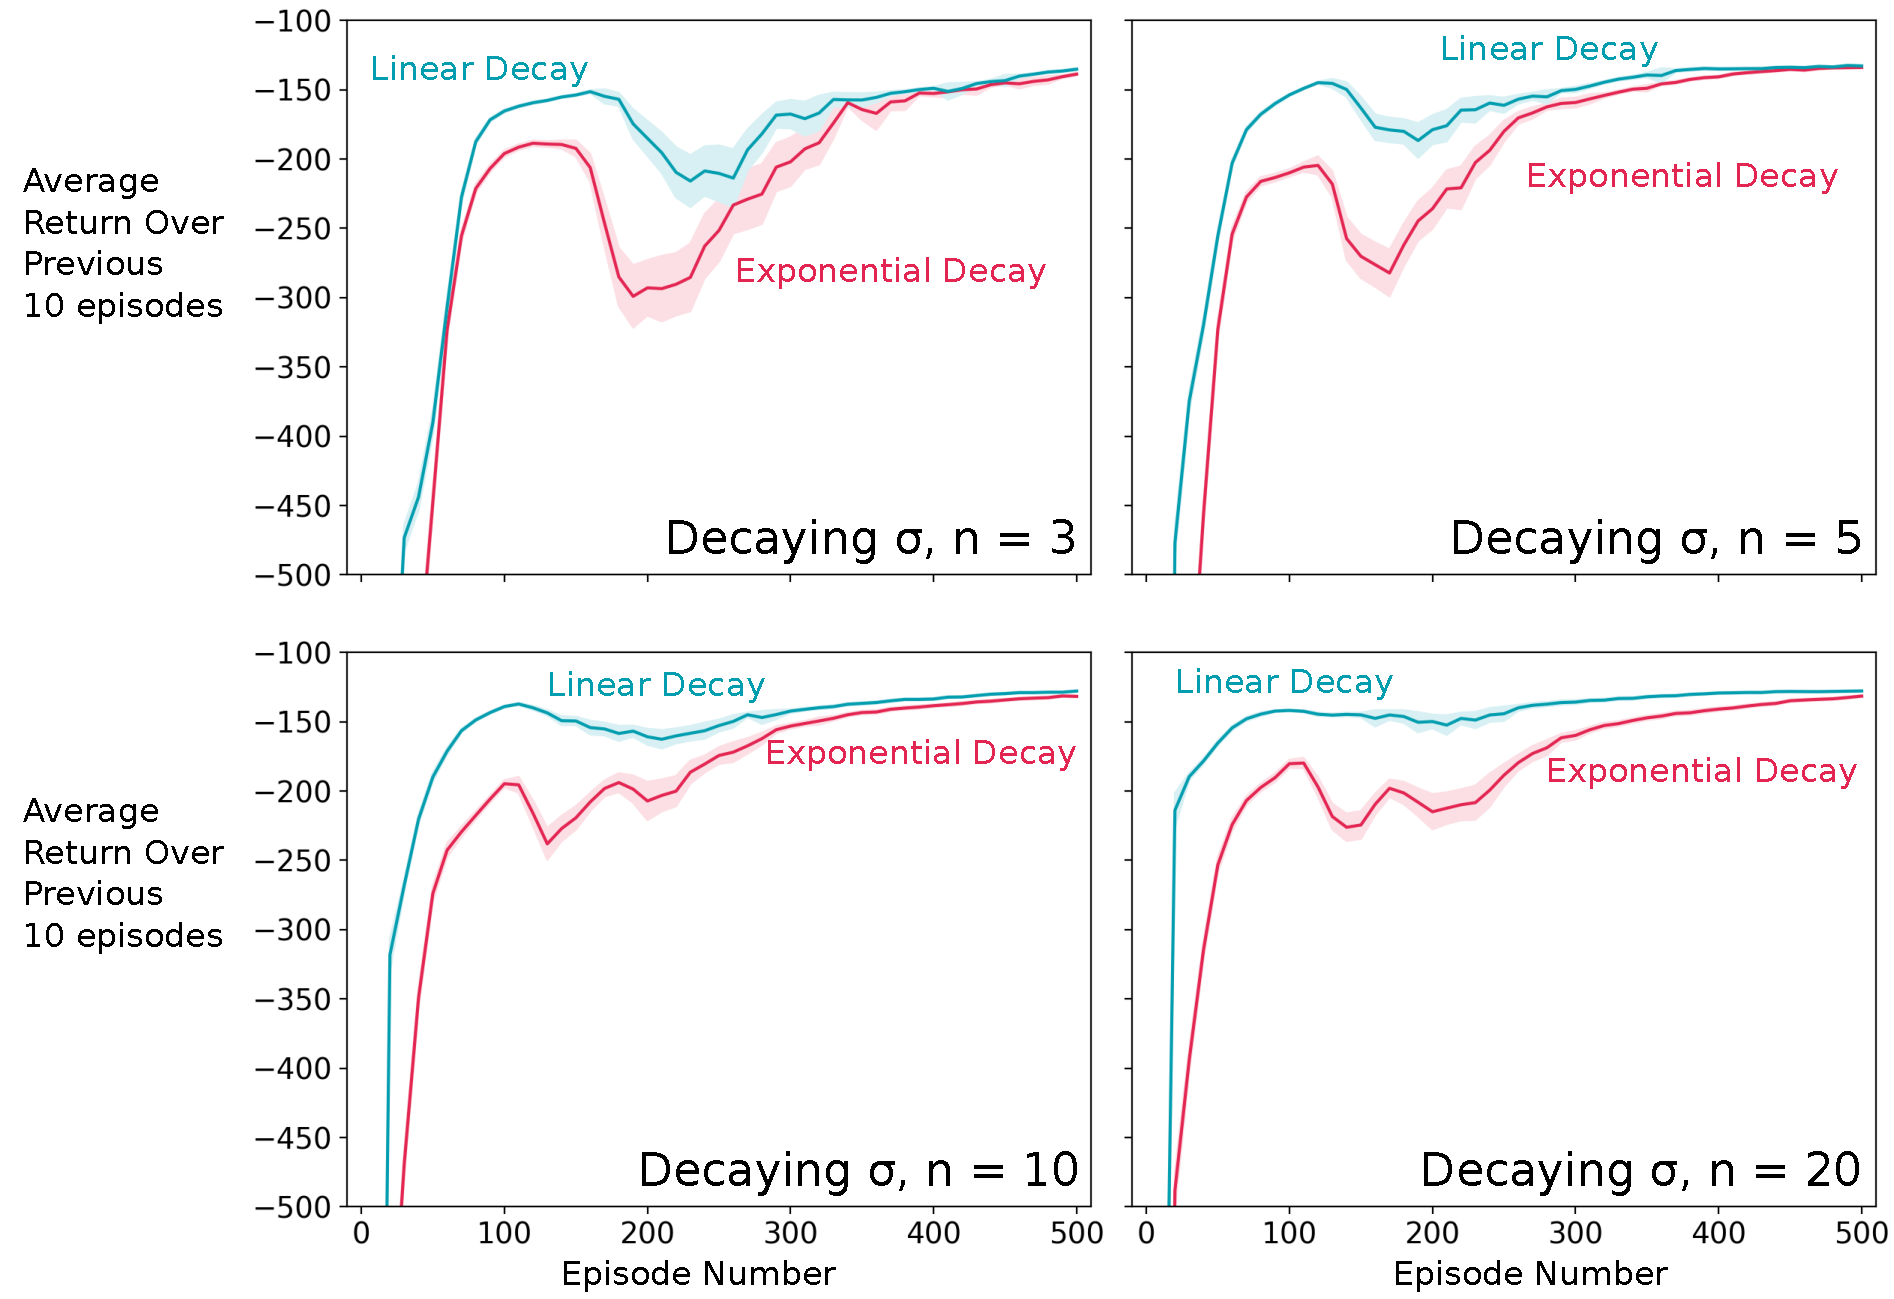
\includegraphics[keepaspectratio=true, width=1\textwidth]{\main/img/decaying_sigma_exponential_vs_linear}
    \caption[Performance of Decaying $\sigma$ with Linear and Exponential Decay] {Performance of decaying $\sigma$ with linear and exponential for several values of $n$.
    The results correspond to the average of $1,000$ independent runs.
    The error bars correspond to a $95\%$ confidence interval.
    Using a linear decay decreased the size of the drop in performance.
    Decaying $\sigma$ performed better with linear decay than with exponential decay.
    }
    \label{fig:linear_vs_exponential}
\end{figure}

The results support our main hypothesis, using a slower decay rate resulted in a smaller drop in performance for decaying $\sigma$ with $n = 3, 5,$ and $20$.
It is reasonable to believe that the same result can be found for $n = 10$ with a larger sample size since decaying $\sigma$ with linear decay has a smaller drop in performance with a $90\%$ confidence level.
By looking at the plots for decaying $\sigma$ with $n = 5$ and $10$, it seems reasonable to extrapolate these results to those algorithms since the exponential decay seems to have a more pronounced drop in both of them.
It possible that the cause of the drop in performance is more complex than we previously thought.
The severity of the drop in performance seem to be an interaction between the back up length and the decay rate. 
For instance, for $n = 3$ the drop in performance was $2$ times smaller when using linear decay than when using exponential decay.
In contrast, for $n = 20$ and linear decay the drop in performance was $4$ times smaller than for the exponential decay.
Thus, it seems that the parameter $n$ amplifies the effect of the decay rate on the drop in performance.

%%%%% Effect of the target network on the performance of the deep $Q(\sigma)$ network %%%%%
\subsection{Effect of the Target Network on the Performance of the Deep $Q(\sigma)$ Network}

There is a possibility that there are more factors influencing the drop in performance experienced by the decaying $\sigma$ algorithm.
A possible candidate is the update frequency of the target network.
During training and in between updates to the target network, the update network --- the network that is updated at every time step --- observes and learns from values of $\sigma$ that the target network has not seen before.
Hence, it is possible that this mismatch in learning between the two networks is inducing some instability in the performance of the decaying $\sigma$ algorithm.
We hypothesized that lower update frequencies for the target network would result in a more stable performance, whereas increasing the update frequency would result in less stable performance.

\begin{table}[t] 
\caption[Comparison of the Sample Standard Deviation of the Average Return per Episode Over 500 Episodes for Decaying $\sigma$ Algorithms with Different Values of the Target Network Update Frequency Parameter]{Comparison of the sample standard deviation of the average return per episode over 500 episodes for decaying $\sigma$ algorithms with different values of the target network update frequency parameter.
The results were computed using $100$ independent runs.
Lower (LB) and upper (UB) 95\% confidence interval bounds computed using a chi-squared distribution are provided to validate the results.
In the linear decay case, lower frequencies result in lower variance for both values of $n$.
}
\label{tbl:variance_analysis}
\begin{center}
\begin{tabular}{lcccc}
\toprule
\multicolumn{5}{c}{Decaying $\sigma$ with Linear Decay} \\
\bottomrule
&& \multicolumn{3}{c}{Average Return per Episode} \\
\cmidrule{3-5}
$n$ & Update Frequency & Standard Deviation & LB & UB \\
\midrule
    & 500       & 21.9      & 19.23     & 25.44     \\
3   & 1,000     & 52.24     & 45.87     & 60.69     \\
    & 2,000     & 106.27    & 93.30     & 123.45    \\ 
\hdashline[3pt/3pt]
    & 500       & 19.63     & 17.24     & 22.81 \\
20  & 1,000     & 40.48     & 35.54     & 47.02 \\
    & 2,000     & 63.38     & 55.65     & 73.63 \\
\bottomrule
&&& \\
\toprule
\multicolumn{5}{c}{Decaying $\sigma$ with Exponential Decay} \\
\bottomrule
&& \multicolumn{3}{c}{Average Return per Episode} \\
\cmidrule{3-5}
$n$ & Update Frequency & Standard Deviation & LB & UB \\
\midrule
    & 500       & 36.12     & 31.71     & 41.96     \\
3   & 1,000     & 85.16     & 74.77     & 98.93     \\
    & 2,000     & 51.96     & 45.63     & 60.37     \\ 
\hdashline[3pt/3pt]
    & 500       & 58.10     & 51.01     & 67.49     \\
20  & 1,000     & 43.75     & 38.41     & 50.82     \\
    & 2,000     & 54.51     & 47.86     & 63.32     \\
\bottomrule
\end{tabular}
\end{center}
\end{table}

To test this hypothesis we implemented decaying $\sigma$ agents with linear and exponential decay with different target network update frequencies taking values in $\{500, 1000, 2000 \}$ and for backup lengths of $3$ and $20$.
This is the only experiment so far that uses a value different from $1,000$ for the target network update frequency.

As a measure of instability in the performance of the algorithm we used the sample standard deviation of the average return per episode over $500$ episodes --- the entire training period.
We computed $95\%$ confidence intervals for the sample standard deviation using a chi-squared distribution.
In this case, the assumptions of the statistical test is that the samples are normally distributed, which is a reasonable assumption in this case since the sample average is normally distributed in the limit.

For decaying $\sigma$ with linear decay, decreasing the the target network update frequency from $2,000$ time steps to $500$ steadily reduced the instability of the algorithm.
On the other hand, for decaying $\sigma$ with exponential decay and $n = 3$, the instability in of the algorithm was the highest with a target network update frequency of $1,000$, the second highest with a frequency of $2,000$, and the lowest with a frequency of $500$.
In the case of decaying $\sigma$ with exponential decay and $n = 20$ there was no difference in the stability of the algorithms for any of the update frequencies. 
The summary of the results are listed in table \ref{tbl:variance_analysis}.

\begin{figure}[t]
    \setlength{\abovecaptionskip}{0pt plus 0pt minus 0pt}
    \centering
    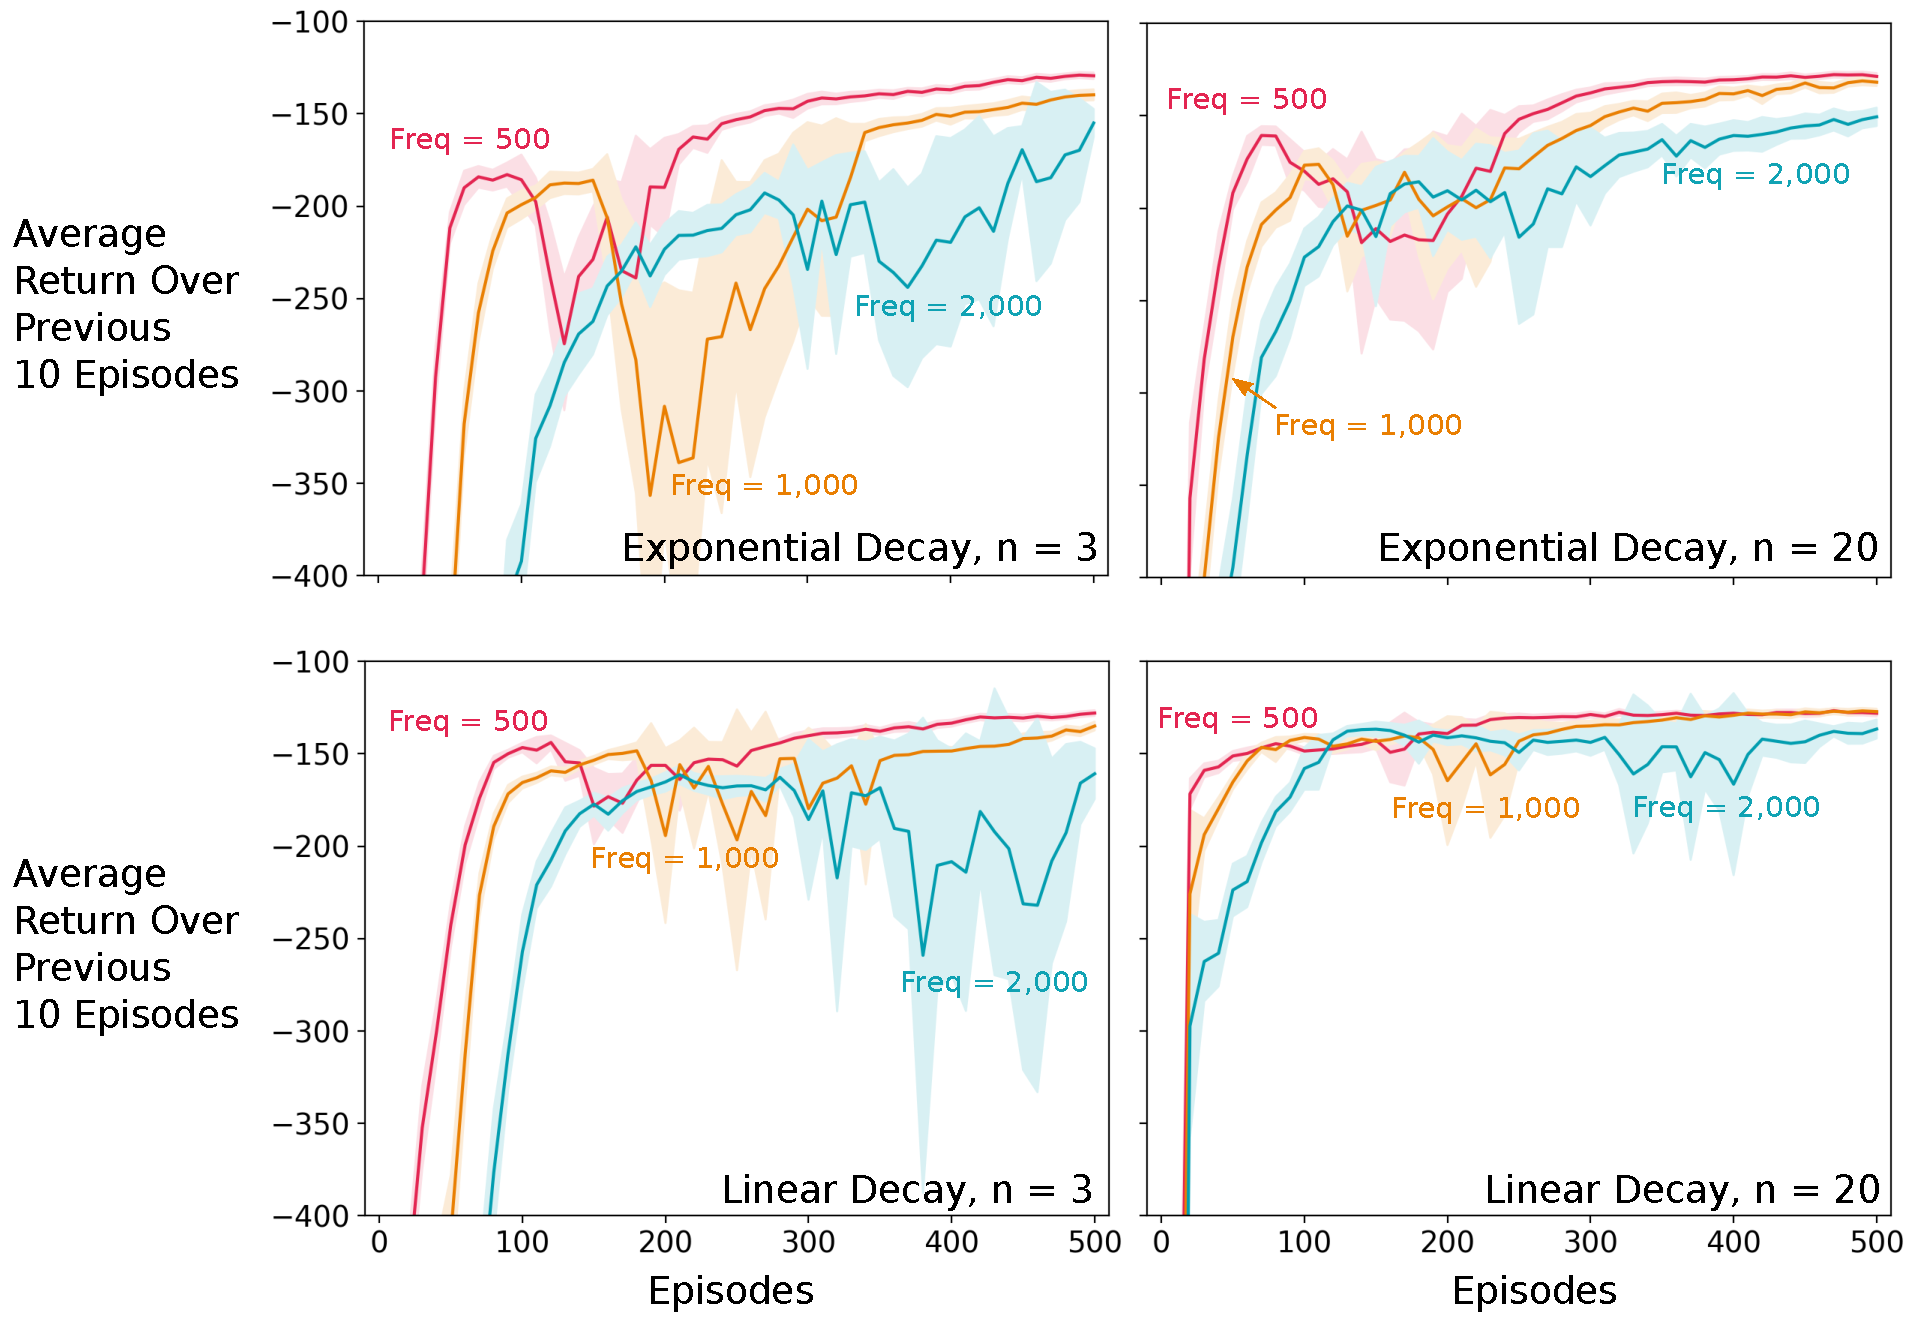
\includegraphics[keepaspectratio=true, width=1\textwidth]{\main/img/tnetwork_ds_comparison}
    \caption[Performance of Decaying $\sigma$ with Different Target Network Update Frequencies] {Performance of decaying $\sigma$ with different target network update frequencies.
    The plot shows the average over 100 independent runs with error bars corresponding to a 95\% confidence interval.
    Smaller update frequencies consistently caused the drop in performance to occur sooner during training.
    }
    \label{fig:tnetwork_ds_comparison}
\end{figure}

Figure \ref{fig:tnetwork_ds_comparison} shows the performance of each algorithm in terms of average return per episode.
The shaded regions correspond to a $95\%$ confidence interval computed using a t-distribution.
It can be seen in the plots that, for the linear decay algorithms, as the target network update frequency increases, the variability of the performance of the algorithm increases.
In the case of the exponential decay, there is no discernible pattern that explains the performance of both values of $n$.

The results of this experiments partially support our main hypothesis.
In the linear decay algorithms, lower values of the target network update frequency resulted in smaller instability, whereas higher values resulted in higher instability.
However, this pattern is not present in the algorithms with exponential decay. 
These results, together with the results from the previous experiment, seem to indicate that the drop in performance of the decaying $\sigma$ algorithm is the result of a complex interaction between the backup length, the decay rate, and the target network update frequency.

%%%%% Effect of the \sigma on the performance of the deep $Q(\sigma)$ network %%%%%
\subsection{Effect of $\sigma$ on the Performance of the Deep $Q(\sigma)$ Network}
\label{subse:ch5_best_nstep}

Now that we have studied how the algorithmic details of the DQN, the parameter $n$, and the decay rate affect the performance of the deep $Q(\sigma)$ network, we move to study the main hypotheses of this section.
Remember that our two main hypotheses were: (1) the decaying $\sigma$ algorithm would perform better than algorithms with fixed $\sigma$, and (2) large values of $\sigma$ would result in better initial performance whereas small values would result in better final performance.

In order to test this hypotheses, we trained four different agents: $Q(0)$, $Q(0.5)$, $Q(1)$, and a decaying $\sigma$ algorithm with a linear decay of $0.002$.
The measure of performance that we used in this experiment was the average return per episode.
To study the initial performance we computed this measure over the first $50$ episodes of training, whereas for the final performance we used the last $50$ episodes of training.
To study the overall performance, we computed this measure over the entire training period --- $500$ episodes.

We only compared the $20$-step versions of each algorithm since they consistently resulted in the best overall performance in the previous experiments.
For each algorithm, we trained $100$ agents for values of the target network update frequency of $500$, $1,000$, and $2,000$, then we selected the value that resulted in the best overall performance.
$Q(0)$, $Q(0.5)$ and decaying $\sigma$ with linear decay performed the best with a target network update frequency of $500$ time steps.
For $Q(1)$, there was no statistical significance between an update frequency of $500$ and $1,000$; nevertheless, we selected $1,000$ since it had the highest average return.

\begin{table}[t] 
\caption[Comparison of the Best Performance of the Deep $Q(\sigma)$ Network with Different Settings of $\sigma$]{Comparison of the best performance of the deep $Q(\sigma)$ network with different settings of $\sigma$.
The standard error, and lower (LB) and upper (UB) 95\% confidence interval bounds are provided to validate the results.
% Decaying $\sigma$ and $Q(1)$ performed the best in terms of initial performance.
% $Q(0.5)$ performed the best in terms of final performance.
% Decaying $\sigma$ performed the best in terms of overall performance.
}
\label{tbl:best_nstep_results}
\begin{center}
\begin{tabular}{lcccc}
\toprule
& \multicolumn{4}{c}{Average Return of First 50 Episodes} \\
\cmidrule{2-5}
Algorithm & Mean & Standard Error & LB & UB \\
\midrule
$Q(1)$, Sarsa 		& \textbf{-297.2}	& 15.79	    & \textbf{-328.52}	& \textbf{-265.88}   \\
$Q(0.5)$  			& -481.6	        & 3.93	    & -489.4	        & -473.8    \\
$Q(0)$, Tree-backup & -647.4	        & 49.32	    & -657.19	        & -637.62   \\
Decaying $\sigma$ 	& \textbf{-273.54}	& 12.103	& \textbf{-297.56}	& \textbf{-249.53}   \\
\bottomrule
&&&& \\
\toprule
& \multicolumn{4}{c}{Average Return of Last 50 Episodes} \\
\cmidrule{2-5}
Algorithm & Mean & Standard Error & LB & UB \\
\midrule
$Q(1)$, Sarsa 		& -130.42	        & 0.81	    & -132.02	        & -128.82   \\
$Q(0.5)$  			& \textbf{-123.78}	& 0.33	    & \textbf{-124.44}	& \textbf{-123.13}   \\
$Q(0)$, Tree-backup & -127.32	        & 0.37	    & -128.06	        & -126.58   \\
Decaying $\sigma$ 	& -127.64	        & 0.39	    & -128.42	        & -126.86   \\
\bottomrule
&&&& \\
\toprule
& \multicolumn{4}{c}{Average Return Over 500 Episodes} \\
\cmidrule{2-5}
Algorithm & Mean & Standard Error & LB & UB \\
\midrule
$Q(1)$, Sarsa 		& -157.05           & 2.18	    & -161.37	        & -152.73   \\
$Q(0.5)$  			& -164.32	        & 0.37	    & -165.06	        & -163.58   \\
$Q(0)$, Tree-backup & -193.73	        & 0.41	    & -194.54	        & -192.92   \\
Decaying $\sigma$ 	& \textbf{-148.46}	& 1.96	    & \textbf{-152.35}	& \textbf{-144.56}   \\
\bottomrule
\end{tabular}
\end{center}
\end{table}

In terms of initial performance, decaying $\sigma$ and $Q(1)$ performed the best --- with no statistically significant difference between their performance, whereas $Q(0)$ performed the worst.
In terms of final performance, $Q(0.5)$ performed the best followed by decaying $\sigma$ and $Q(0)$ --- there was no statistically significant difference between their performance; and $Q(1)$ performed the worst.
Finally, considering the whole training period, decaying $\sigma$ performed the best among all the algorithms followed by $Q(1)$ as a close second, then $Q(0.5)$, and at last $Q(0)$.
Table \ref{tbl:best_nstep_results} shows the summaries of $100$ independent runs for the initial, final, and overall performance for all the algorithms.
Figure \ref{fig:best_nstep} shows the performance during training at intervals of $50$ episodes for each algorithm.
The error bars correspond to a $95\%$ confidence interval.


\begin{figure}[t]
    \setlength{\abovecaptionskip}{0pt plus 0pt minus 0pt}
    \centering
    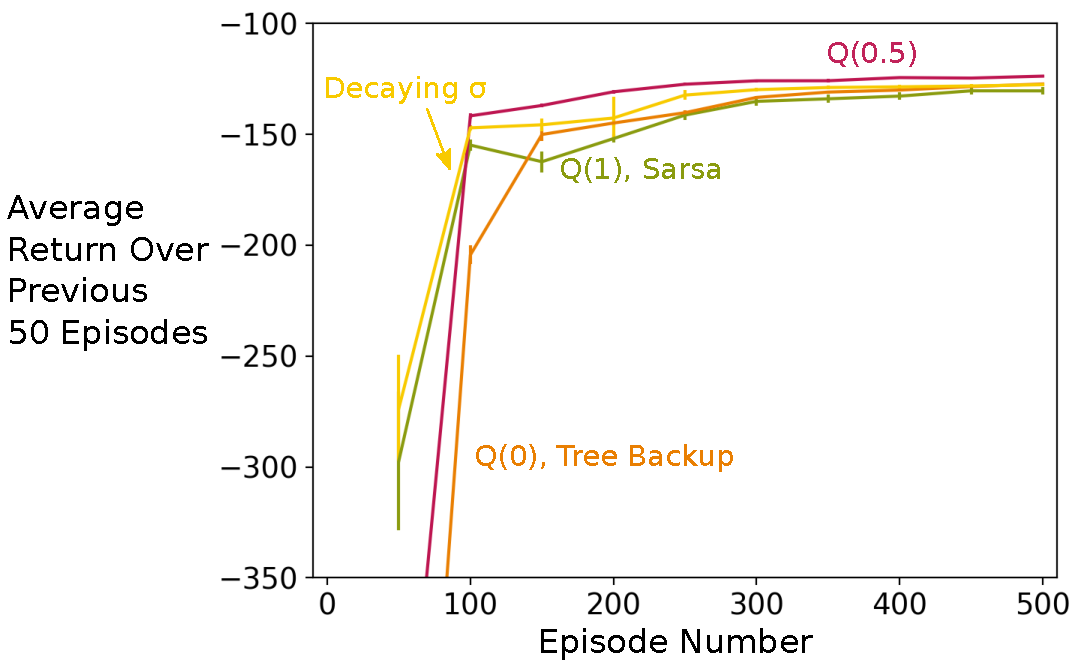
\includegraphics[keepaspectratio=true, width=1\textwidth]{\main/img/best_nstep_comparison}
    \caption[Comparison of the Deep $Q(\sigma)$ Network Algorithms with the Best Performance for Different Values of $\sigma$] {Comparison of the deep $Q(\sigma)$ network algorithms with the best performance for different values of $\sigma$.
    The plot shows the average over 100 independent runs with error bars corresponding to a 95\% confidence interval.
    Sarsa and decaying $\sigma$ with linear decay had the best initial performance among the four algorithms. 
    $Q(0.5)$ had the best final performance followed closely by decaying $\sigma$ with linear decay and tree backup.
    }
    \label{fig:best_nstep}
\end{figure}

The results partially support our hypotheses.
Decaying $\sigma$ performed the best in terms of overall performance.
Nevertheless, it tied with $Q(1)$ in terms of initial performance and it tied for second place with $Q(0)$ in terms of final performance.
$Q(0.5)$ did not have the best performance during early training, however, after $100$ episodes of training, it consistently had the best performance among all the algorithms.
Hence, it seems possible to improve the final performance of decaying $\sigma$ by letting the final value of $\sigma$ be $0.5$ instead of $0$.

For the second hypothesis, increasing the value of $\sigma$ consistently improved the initial performance.
However, decreasing the value of $\sigma$ did not consistently improve the final performance.
The evidence indicates that the best final performance is attained at some intermediate value of $\sigma$ possibly close to $0.5$. 

Lastly, one interesting observation from the optimization of these algorithms is that decreasing the target network update frequency improved the performance of $Q(0.5)$ and $Q(0)$.
This implies that, similar to decaying $\sigma$, the mismatch in learning between the update network and the target network hinders the performance of these algorithms.
To see the full summary of the these algorithms with different target network update frequencies see appendix (APPENDIX A).

%%%%%%%%%%%%%%%%%%%%
%%%%% Summary  %%%%%
%%%%%%%%%%%%%%%%%%%%
\section{Summary}

In this chapter, we have accumulated increasing evidence to support the claim that there is a benefit in using $n$-step $Q(\sigma)$ over the $n$-step algorithms Sarsa and tree backup.

We demonstrated that decaying $\sigma$ --- a version of $n$-step $Q(\sigma)$ were $\sigma$ decays from $1$ to $0$ over time --- performs better in terms of overall performance than any of the $n$-step $Q(\sigma)$ algorithms with fixed values of $\sigma$.
This result seems to be robust to different environments and different representations of the action-value function.
Moreover, we also found in several of our experiments that algorithms with intermediate values of $\sigma$ also performed better than algorithms using $\sigma$ equal to $1$ (Sarsa) or $0$ (tree backup).

The parameter $\sigma$ seems to influence the performance of the $n$-step $Q(\sigma)$ algorithm during early and late training.
In the $19$-state random walk environment, we found that increasing the value of $\sigma$ from $0$ to $1$ improved the initial performance but worsen the final performance.
%% maybe revise this sentence(?)
This effect 
% of that the parameter $\sigma$ has on the initial and final performance 
seems to be affected by the type of environment and the type of representation used for the action-value function.
%%
In the mountain cliff environment with linear function approximation we found that the best \textbf{initial performance} was achieved with a value of $\sigma$ of $0.5$ and the initial performance worsen the farther away $\sigma$ was from this value.
Nevertheless, we still found that as the value of $\sigma$ decreased from $1$ to $0$ the resulting algorithms consistently performed better during late training.
In contrast, when using non-linear function approximation in the mountain car environment, we found that the best \textbf{final performance} was achieved with a value of $\sigma$ of $0.5$ and the final performance worsen the farther away $\sigma$ was from this value.
Moreover, we found that as the value of $\sigma$ increased from $0$ to $1$ the resulting algorithms performed better during early training.

The behaviour of $n$-step $Q(\sigma)$ algorithm, including $Q(1)$ (Sarsa) and $Q(0)$ (tree backup), changed significantly depending on the learning problem, the environment, and the type of representation used for the action-value function.
Nevertheless, we were always able to adapt the $n$-step $Q(\sigma)$ algorithm in order to improve its performance in every single one of the tasks studied in this chapter.
This would not have been possible if not for the parameter $\sigma$.
Therefore, the main benefit of using $n$-step $Q(\sigma)$ is the flexibility that it provides and that allows it to be adaptable to the particular characteristics of the learning task.

\end{document}